\chapter{Threat Intelligence Uses}
\label{chapter:data_usage}

In the last chapter, I talked about the data characteristic of 
existing Threat Intelligence products and their limitations. Given
the current status of Threat Intelligence, another side of the coin is:
how people are actually using the data currently. This question belong 
to the empirical study on data operation, as I listed in the 
introduction chapter.

As one can see, threat intelligence data can be used in a number
of different ways. It can be used forensically during incident response
(i.e., to better understand and attribute a threat after it has gained
access to a network), it can be used reactively to generate alerts
of suspicious activity in a SIEM system. 
(i.e., to raise awareness of a potential threat
that is currently active), or it can be used proactively to block
traffic (and hence block the associated threats). This last category
of action, traditionally called ``blacklisting'', is uniquely
attractive to a defender since, if effective, it can foreclose certain
threats without requiring individualized attention from a human
analyst. Indeed, it is common to see such precise scenarios
highlighted in the marketing materials for virtually all threat
intelligence offerings.

%However, it far from clear if this promise of threat intelligence in
%the abstract is matched by its implementation in practice.
However, despite all the promises, it is far from clear how people 
actually adopt threat intelligence data, especially for proactive
traffic blocking. Proactively blocking traffic based on threat 
intelligence data is a strong action, and as I showed in last chapter,
threat intelligence feeds can be far from comprehensive and may include
significant numbers of false positives. This could cause an organization
to inadvertently block benign Internet sites. Moreover, on a broader 
scale, a mistakenly added IP in a threat intelligence feed can
effectively be denied service from all organizations using that feed
to block traffic. Given this, it is important to understand the extent
to which network administrators are willing to use such third-party data 
to block network traffic.

In this chapter, I will take the first step towards understanding this
question. In particular, this study seeks to better understand the extent 
to which network administrators make use of threat intelligence IP feeds
(more commonly known as IP blacklists) to proactively block network 
traffic and, if they do, which kinds of data sources are they using for 
that purpose.

The principal challenge in pursuing this question is that such
decisions are largely invisible: a network choosing to block IP
address x, is indistinguishable from one that does not, except to the
owner of IP address x.  Moreover, for operational security reasons,
few organizations are willing to publicly document the details of
their network defenses. Thus, there is no crisp mechanism to
determine if a network blocks certain traffic, let alone a means to
determine the data source driving such a decision.

In this chapter, I explore this question via a combination of inference
and careful testing, resulting in three primary contributions.
First, building on prior work designed to detect
censorship~\cite{ensafi2014detecting, pearce2017augur}, I develop,
test and validate an inference technique using the IP ID side-channel to
detect network-layer blacklisting.  Second, by using this technique with 
a carefully chosen set of IP addresses, I am able to attribute
blocking actions to the use of particular blacklists. Finally, I conduct 
a large-scale pilot study covering over {\reflroughnum} U.S. hosts
to explore the diversity in blacklisting behaviors. Together, this work
uncovers the use of {\blacklistnum} popular public IP blacklists among
the hosts I surveyed, and demonstrate relations between these hosts
and their update pattern on blacklists. I further investigate a broader
use of blacklists among the hosts, and discovered over 73K hosts has
shown blacklist related blocking behavior.


\section{Technical Background}

\subsection{Internet Connection Blocking}
In this work, I focus on one specific way of how organizations are using 
threat intelligence data: use threat intelligence IP feeds as direct rule-set 
to block network traffic. This behavior is very similar to other forms of
Internet connection blocking, most notable examples are Internet censorship,
geo-blocking and Tor blocking.

Many previous work has studied Internet censorship~\cite{aryan2013internet,
park2010empirical,anderson2012splinternet,zittrain2003internet,
clayton2006ignoring}, geo-blocking~\cite{opennetsurvey, mcdonald2018403,afroz2018exploring}, 
and Tor blocking~\cite{singh2017characterizing, khattak2016you}. However, 
these measurement studies all rely on having vantage points in the target 
regions, so the researchers can directly measure the network effects and 
acquire the results. There are serval public projects that facility such 
studies by providing access points around the global, like RIPE
Atlas~\cite{ripeatlas}, OONI~\cite{ooni} and ICLab~\cite{iclab}.
For Tor blocking, it is also not hard for the researchers to get access 
to a Tor exit node~\cite{khattak2016you}, then conduct the following 
measurement from that node. But these studies are restrained by the vantage
points they could get, as it is hard to get these vantage points in large
quantities, and these points are also heavily biased towards certain networks.
For country-wide censorship or geo-blocking measurement, this is not a big
issue. But in this case, I want to conduct large scale measurements over a 
broad set of online hosts, it is very difficult to acquire vantage points 
that can meet my requirements.

Recent work by Ensafi et al~\cite{ensafi2014detecting} and Pearce et 
al~\cite{pearce2017augur}. demonstrated the method to use IP ID side 
channel to measure Internet connectivity. This is an indirect method 
and allow an observer to measurement the connectivity between two hosts 
without having access to either of the hosts. In this study, I do not 
have access to either threat intelligence feeds, or large amount of 
online hosts, this method is an ideal method for this measurement. But 
I need to modify the original method to better suit this experiment, 
and I also need to take extra effort to eliminate the interfering 
signals. I will establish on the methodology in more detail in
Section~\ref{sec:methodology}.

% First Paragraph: Explain what is IP ID
\subsection{IP ID Side Channel}
\label{sec:ipidchannel}
The Identification (ID) field of an IPv4 packet is a 16-bit value in the IP
packet header. It is designed primarily to support IP packet fragmentation
and reassembly. If a large IP packet is fragmented when sent through the
network, the receiving end will use this field to identify the fragments from
the same IP packet and re-assemble them. This requires the 16-bit value to be
unique for every datagram of a given source address, destination address, and
protocol, such that it does not repeat within the maximum datagram
lifetime~\cite{postel1981rfc0791}.

% Second paragraph: how a lot of people are implementing it.
One easy way to implement the IP ID field for networking is to use a global
counter. In this case, a system uses one 16-bit variable to set the IP ID
value for all the IP packets it sends out, and increments the variable by 1
after every packet. This simple solution ensures the IP ID value of all
packets are unique, and it is how many early systems implemented their
IP ID mechanisms~\cite{klein2019ip}.

This implementation create a side channel that allows anyone without
access to a host to observe the traffic volume from that host. An observer,
by probing the host twice separated by some time interval and checking the
corresponding IP ID increase, can learn about the number of packets the host
sent out during this period. This side channel can be used to observe many
different network effects, like host alias detection~\cite{spring2002measuring},
where observers can detect if two online hosts actually correspond to one 
physical machine by monitoring their IP ID changes, and NATed host 
counting~\cite{bellovin2002technique}, where observers can identify the 
number of machines behind a NAT by tracking the number of IP ID sequences 
from the packets comming out of the network.

In order to eliminate this side channel, new systems implement the IP ID
generation by using different counters for different traffic, so different
observers will see a different IP ID sequences from the same host. However,
there are still a significant number of hosts on the Internet that still use
the global counter implementation. For example, Windows 8 and older still use
this implementation~\cite{klein2019ip}. These hosts give us sizable amount of
candidates to conduct this measurement.
\mathchardef\mhyphen="2D % Define a "math hyphen"

\section{Methodology}
\label{sec:methodology}

In this chapter, I use the IP ID side channel (Section~\ref{sec:ipidchannel})
to determine whether a particular online host blocks traffic using one
or more known blacklists. In brief, I begin by identifying hosts that are
suitable for this technique. I refer to such hosts as
\emph{reflectors}. Then I randomly sample a set of IP addresses
from IP blacklists that could be used to block traffic. Such IP addresses 
will be refered as \emph{blacklist IPs}. Then I measure if
each reflector blocks packets whose source addresses are blacklist
IPs. If one reflector blocks all IP addresses I sampled
from one particular blacklist, then it is probably using that blacklist.

In this section, I first describe how the technique works at a
high-level (Section~\ref{sec:meththeory}). Then I detail
the method for identifying proper {\reflectors} for the
measurement (Section~\ref{sec:methrefl}), how to choose target blacklists 
to test (Section~\ref{sec:methblkl}), and how to sample IP addresses from 
each blacklist (Section~\ref{sec:methtarg}). In Section~\ref{sec:methtrain}, 
I explain the experiment design in detail and how it works in
real world scenarios. Section~\ref{sec:methvalid} further describes the steps
I take for sanity check, and in Section~\ref{sec:ethics} I discuss the
ethical considerations of the methodology.

\subsection{Technique Overview}
\label{sec:meththeory}

To measure if one {\reflector} is blocking one particular IP from a blacklist,
I send a train of packets (here I use SYN-ACK packets)
from the measurement machine to the {\reflector}. The packet train consists
of packets whose source address is the blacklist IP (spoofed),
bracketed by packets whose source address is the measurement machine,
as illustrated in Figure~\ref{fig:coreidea}. If a firewall in the
reflector's network blocks packets from the blacklist IP, the
reflector will not receive packets with the blacklisted source address. In
this case, it will only receive packets with the measurement machine's source
address. On the other hand, if there is no firewall blocking such packets, the
reflector will receive the entire packet train.

%a variation of the Ensafi technique proposed for censorship
%measurement~\cite{ensafi2014detecting}.

\begin{figure}[t]
    \centering
    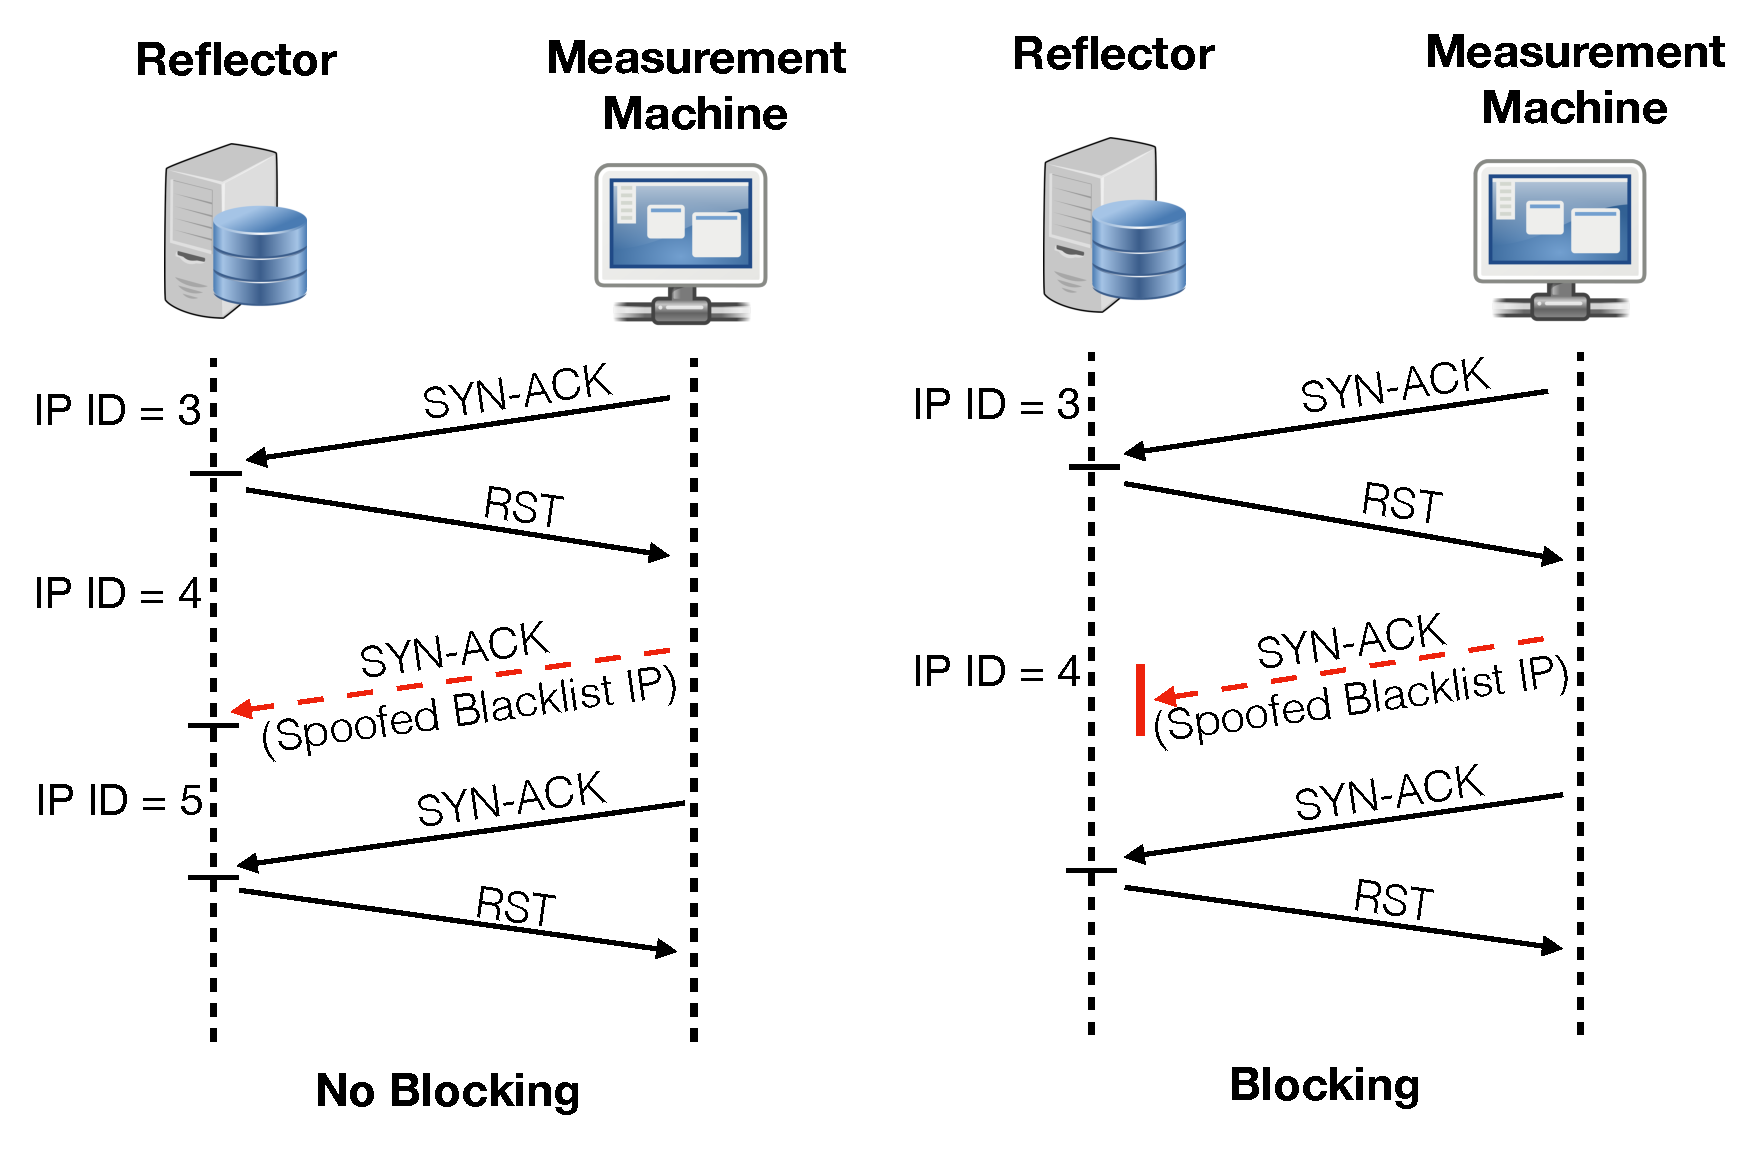
\includegraphics[width=0.98\columnwidth]{data_usage/images/cropped_method_protocol_v2.pdf}
    \caption{The basic method to detect network blocking using the IP ID side channel.}
    \label{fig:coreidea}
\end{figure}

In an ideal world, where there is no packet loss during transmission
and no extra traffic on the {\reflector}, one would see a clear difference
in the IP IDs from the responses between the two different scenarios.
In particular, I expect the {\reflector} to send a RST response for
each SYN-ACK packet I send, and I will receive the responses for
the SYN-ACK with the measurement machine's source address. The IP IDs of 
these received RST packets will reflect the number of packets sent by the
reflector. If the reflector did not receive the SYN-ACK packets with the
blacklist IP as source addresses(because they were blocked by a
firewall), the IP ID sequence in the RST responses will be an
increasing sequence without gaps (the ``Blocking'' case in Figure~\ref{fig:coreidea}).
On the other hand, if the reflector did
receive the SYN-ACK packets with the blacklist IP, it would have sent
a RST packet in response to each such packet, incrementing the IP ID counter
each time. While I will not see the RST packets sent to the blacklist
IP, I \emph{will} observe the increments in the IP ID sequence.
More specifically, one would see a gap in the IP ID sequence of packets
received by the measurement machine (the ``No Blocking'' case in
Figure~\ref{fig:coreidea}).
These two cases, illustrated in Figure~\ref{fig:coreidea}, allow us to
determine whether a particular blacklist IP is blocked by some network
device, such as a firewall, somewhere between the measurement host and
the reflector. When there is no blocking in place (left), the measurement
machine will see an IP ID gap in two RST responses: the second IP ID will
increase by two. Whereas if there is network blocking (right), then the
two IP IDs will not have a gap: the second IP ID will only increase by
one.
%and this gap should equal the number of RST
%packets sent to the blacklisted addresses, which, in turn, should equal the
%number of SYN-ACK packets received by the reflected with the blacklisted
%address.

This measurement technique is inspired by the method proposed in previous
work~\cite{ensafi2014detecting, pearce2017augur}. However, to make it work 
for my objective I need to handle a few more important issues, as I will
see in the rest of this section.

\subsection{Compare with Previous Method}

At a high level, the objective of the measurement is to determine, from a third
point, if a {\reflector} blocks a blacklist IP. The blocking behavior that we
want to measure is \textit{inbound blocking} -- that is the incoming traffic
is blocked and as a result traffic does not reach the intended host. A
typical example is a network firewall, where it can stop certain network
packets from reaching hosts behind the firewall. Here we abstract the
{\reflector} as $Host_A$, blacklist IP as $Host_B$, and the problem is to
detect the connectivity between two hosts on the Internet.

%Another type of blocking is %\textit{outbound blocking}, where the outgoing
%traffic to a ``blocked host'' from a host within the network is blocked. %A
%typical example is network censorship. Our measurement in this paper only
%focuses on inbound blocking, %and we will explain more about this in the
%following sections.

\begin{figure}[t]
\centering
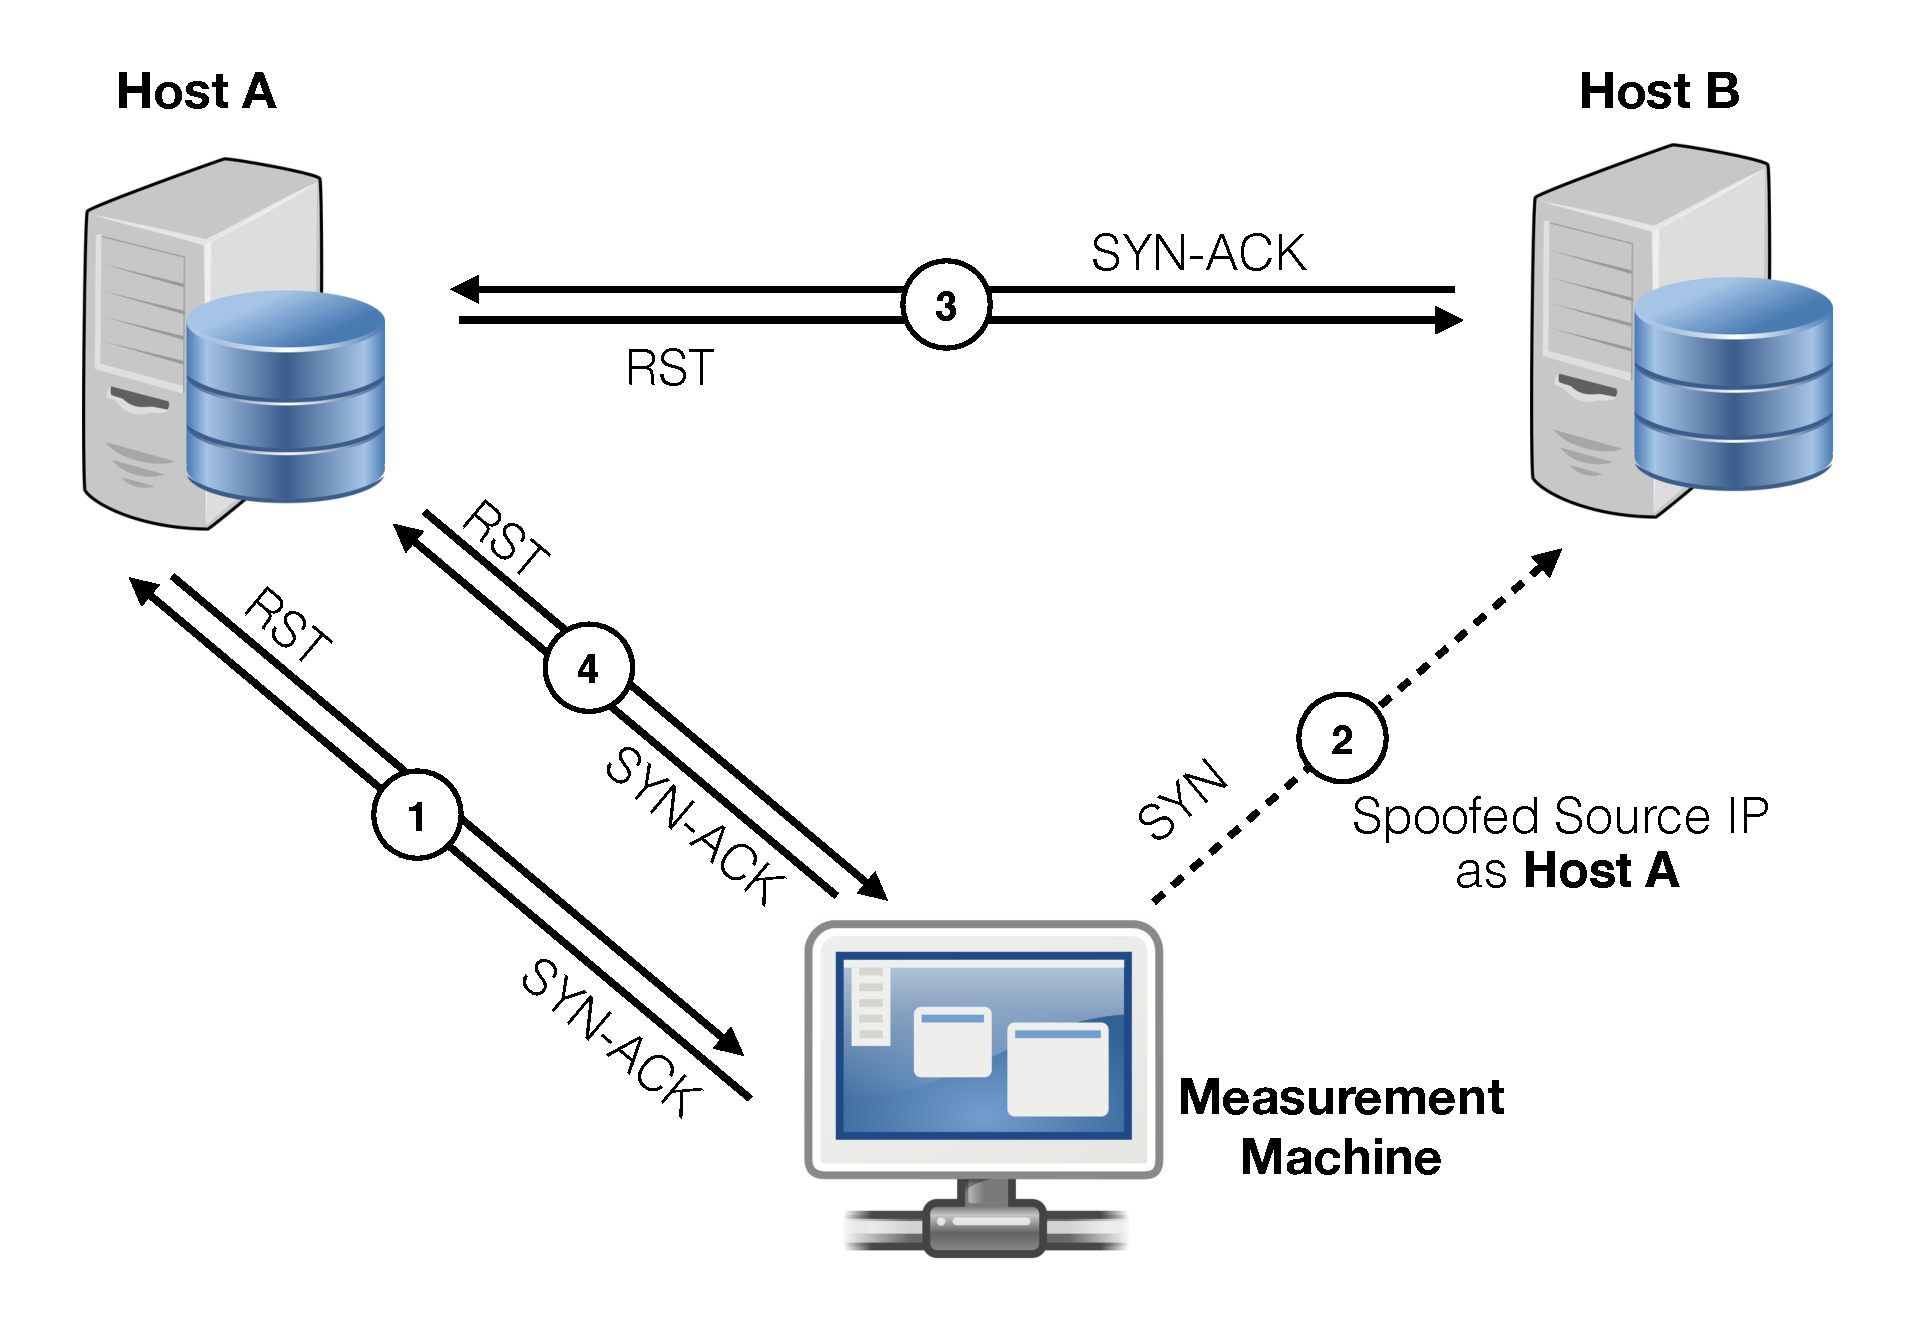
\includegraphics[width=0.8\columnwidth]{data_usage/images/croped_method_old.pdf}
\caption{Measurement method used in previous work.}
\label{fig:old_method}
\end{figure}

In previous works~\cite{pearce2017augur, ensafi2014detecting}, to measure
the connectivity between two hosts from a third party, they send spoofed packets
to impersonate one of the hosts. This methodology -- one we refer
to as the \textit{triangle measurement} takes advantage of the TCP 3-way
handshake protocol, as shown in Figure~\ref{fig:old_method}.

The measurement machine first sends a probe to the $Host_A$, in this case a TCP
SYN-ACK packet. $Host_A$ responds with a RST packet since it received a SYN-ACK
without the preceding SYN packet. Thus, the measurement machine gets the
first IP ID $IP\mhyphen ID_1$ from the RST packet (corresponds to Step 1 in
the figure). Next, the measurement machine sends a spoofed TCP SYN packet to
$Host_B$, with source IP address set to the IP address of $Host_A$ (Step 2).
$Host_B$ then sends a responding SYN-ACK packet to $Host_A$, which causes $Host_A$
to respond with a RST packet (Step 3), and increment its IP ID counter by 1.
Finally, the measurement machine probe $Host_A$ again and get the second IP ID
$IP\mhyphen ID_2$ (Step 4).

Now we can infer whether $Host_A$ is inbound blocking traffic from $Host_B$ by
observing the difference between $IP\mhyphen ID_1$ and $IP\mhyphen ID_2$.
Assuming there is no packet loss, and that $Host_A$ does not have any extra
traffic besides our measurement traffic, then
$IP\mhyphen ID_2 = IP\mhyphen ID_1 + 2$ implies there is no inbound blocking,
since it indicates that $Host_A$ received both packets in step 3 and step 4,
while $IP\mhyphen ID_2 = IP\mhyphen ID_1 + 1$ means there is blocking.

Previous work chose this ``triangle measurement'' because it ensures that in
step 3, the packets from $Host_B$ will go through the same routes as the
traffic originated from $Host_B$. So from $Host_A$'s perspective, it can not
identify that the traffic from $Host_B$ are spoofed. However, in this schema,
one hard requirement is that $Host_B$ needs to be active and responding to TCP
SYN probe. This is not an issue for censorship measurement, as $Host_B$ in this
case are popular sites (Google, Facebook, Twitter etc.) that guaranteed will
respond to SYN probe.

However, in our case, we need to measure whether $Host_A$ is blocking traffic
from a blacklist IP($Host_B$). But there is no guarantee that these IP
addresses are active and thus may not respond to our SYN probe. In fact, we
found that the percentage of responding IPs in a blacklist can be as low as less
than 20\%. This dramatically reduces the candidate IPs we can sample from a
blacklist to test, especially for small blacklists that only have a few hundred
IPs. Furthermore, there are many other additional constraints when shortlisting
IPs for measurement from a blacklist.
The requirement that blacklist IPs respond to SYN probe does not work for our
use case. 
%\textcolor{red}{Explain the choice for only inbound blocking}

In order to get around this limitation we adjust the measurement methodology.
In this new methodology, the measurement machine directly sends spoofed
packets to the target host, as shown in Figure~\ref{fig:new_method}. In
this case, the measurement machine first probes $Host_A$ to get the first IP ID
$IP\mhyphen ID_1$, then it sends a spoofed packet, with source IP set to
$Host_B$(Blacklist IP), directly to $Host_A$. Finally, it sends a second probe
to $Host_A$ and get the second IP ID $IP\mhyphen ID_2$. Now we can use the same
logic as before to infer whether $Host_A$ is inbound blocking $Host_B$. In this
approach, we do not require $Host_B$ to be actively responding SYN packets, any
IP address can be used here to conduct the test. The drawback is that the
spoofed packets now at times go through a different route versus the packets
originated from $Host_B$. Some network that implement spoofed packet
detection~\cite{ferguson2000rfc2827} could drop our spoofed packets, giving us
a false signal of inbound blocking. Therefore, when selecting hosts we conduct
extensive tests to weed out hosts that have such detection logic in place. We
find that not a lot of target hosts have such detection logic. We will talk in
detail about host selection in the follow sections.

%Therefore, we modified the measurement so that the measurement machine  directly
%send spoofed packets to host A, as shown in Figure~\ref{fig:new_method}. In
%this case, the measurement machine first probes host A to get the first IP ID
%\texttt{IP\_ID\_1}, then it sends a spoofed packet, with source IP as host B,
%directly to A. Finally, it sends a second probe to host A and get the second
%IP ID \texttt{IP\_ID\_2}. Now we can use the same logic as before to infer
%whether host A is inbound blocking host B. In this approach, we do not
%require host B to be actively responding SYN packets, any IP address can be
%used here to conduct the test. The drawback now is that the spoofed packets
%will likely go through a different route versus the packets originated from
%host B. Some network that implemented spoofed packet detection~\cite{ferguson2000rfc2827}
%could drop our spoofed packets, giving us a false
%signal of inbound blocking. Therefore, when selecting hosts for the
%measurement, we conduct extensive tests to make sure the hosts do not have
%such detection logic in place. Our experiment also shows that not a lot of
%hosts have such detection logic. We will talk in detail about host selection
%in Section~\ref{sec:requirement_host}.

\begin{figure}[t]
\centering
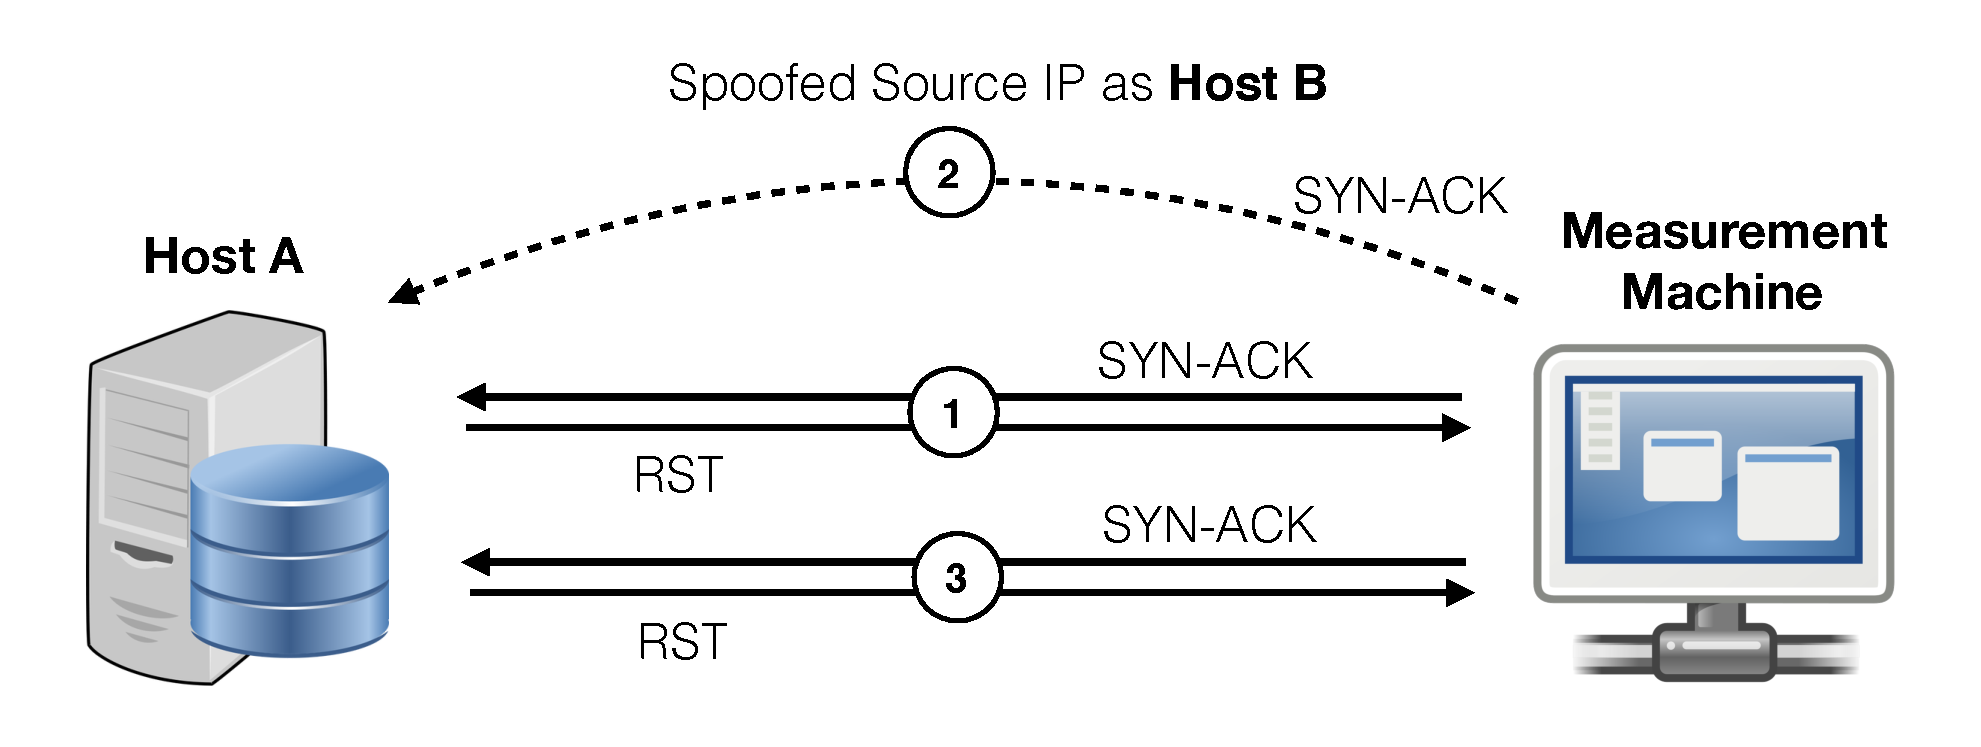
\includegraphics[width=0.8\columnwidth]{data_usage/images/croped_method_new.pdf}
\caption{Measurement method used in this work.}
\label{fig:new_method}
\end{figure}

\subsection{Finding Suitable Reflectors}
\label{sec:methrefl}

At a high level, my methodology relies on being able to infer blocking
using the IP ID side channel. Keeping that in mind, listed below is the
criteria I look for when scanning the Internet to search for suitable
reflectors.

\begin{itemize}
    \item \textbf{RST packet generation:}
    The {\reflectors} must reply with a RST packet to a TCP SYN-ACK packet 
    without an established connection. Some hosts drop incoming SYN-ACK 
    packets if there is no corresponding SYN packet. These hosts are not
    suitable for my measurement methodology. I choose SYN-ACK packets 
    instead of SYN because it does not create an intermediate state on the
    {\reflectors} and connection is terminated in one go.

    \item \textbf{Shared monotonic increasing IP ID counter:}
    The IP ID counter in the {\reflector} needs to be globally shared, so all
    network traffic generated from the host will use the same counter for IP
    ID assigning. It also needs to be monotonically increasing, so I can
    observe the number of packets generated by the host between two
    measurements using the difference of IP IDs.
    
    \item \textbf{Low traffic:}
    The technique requires the host to have low traffic volumes
    in general, since the technique depends on the fact
    that I can observe a clear difference in IP ID increases when sending
    spoofed packets. If there are always many other
    packets coming to the host, it would be infeasible to observe the IP ID
    changes triggered by the measurement packets.

    \item \textbf{No ingress filtering:}
    I send spoofed packets to {\reflectors} to infer traffic blocking.
    However, some network providers utilize ingress filtering techniques and
    drop packets once they detect the packets are not from the networks they
    claimed to originate. This would cause the spoofed packets being dropped
    and give us a false signal of traffic blocking.

    \item \textbf{No stateful firewall blocking:}
    Some networks deploy a stateful firewall that blocks access from a source
    IP after receiving too many repetitive packets. One example is to defend
    against SYN floods~\cite{lemon2002resisting}. While I try to keep the
    number of the measurement packets as low as possible, if the spoofed
    packets trigger such firewall rules and then I are blocked by the 
    firewall, I will incorrectly conclude that the {\reflector} uses a
    blacklist to block that IP.
\end{itemize}

I try to uncover how online hosts are using IP blacklists to
block traffic. But when looking at the problem on a global scale, there are
many policy related reasons why a host blocks network traffic,
such as censorship. These alternate sources of blocking could disrupt the
measurement, making it hard to distinguish the type of security-related 
blocking I target. To simplify the problem, in this chapter I focus on 
the hosts in United States.

I find {\reflectors} in the United States with open ports using a snapshot
of Censys~\cite{censys} scanning data from November 8, 2019. Then I scan 
these 40 million hosts to identify the ones with the IP ID side channel. 
I send multiple probes to each host targeting an open port from different
source addresses, and then check IP IDs in the responses. In the case where 
hosts have multiple open ports, I randomly select a port to send the probe.

To identify stateful firewalls, I send SYN-ACK packets to each {\reflector}
in two different patterns: 1 second per packet with 24 packets, and 5 packets
per second with 60 packets, which corresponds to the speed I probe
{\reflectors} during actually experiments (see the following section). I
repeat each experiment 6 times and discard the hosts that block us after the
experiment. To find the hosts with low extra traffic, I send 24 probes
to each host, 1 per second, and repeat the experiment 5 times at different
times of the day. I then collect the result and only select the hosts where
more than 30\% of their IP ID increases are equal to 1 per second --- that is,
the host did not receive any extra traffic besides my probes,
and all of the increases were smaller than 10 within a second.

Finally, I try to identify hosts experiencing ingress filtering. To
account for differences in ingress filtering that may possibly occur on
different network paths to the {\reflectors}, I acquired 7 vantage points 
around the world to exercise different paths. These vantage points are
from the US west coast, east coast and midwest, and places in Asia, Europe,
Australia and South America.

I then send spoofed packets from my measurement
machine to the {\reflectors} with spoofed source addresses corresponding to
the 7 vantage points, and later collect responses at each vantage point.
I only select the {\reflectors} that send responses to all 7
vantage points, meaning they did not drop spoofed packets on these network paths.

Eventually, I identified {\reflcount} IP addresses in US that meet the
requirements.\footnote{I initially discovered more than 300K {\reflectors}, 
but during my experiments some hosts became inactive. The number reported 
here is the final number after I finished all the experiments.} For the 
purpose of this chapter, here I treat each individual IP address as a 
distinct {\reflector}. Detailed numbers are presented in
Table~\ref{tab:target-hosts}.

\begin{table}[t]
\centering
\caption{The number of {\reflectors} (IP addresses) identified in the United States, and the
corresponding count of /24 prefixes and Autonomous Systems.}
\begin{tabular}{l >{\hfill}p{4.5cm}}
 \toprule
 Category                    &  Count    \\
 \midrule
 \textbf{IP Addresses}       &  \reflcount  \\
 \textbf{/24 Count}          &  128,712  \\
 \textbf{Autonomous Systems} &  3,371    \\
%% \textbf{Organizations}      &  3,321    \\
 \bottomrule
\end{tabular}
%% and organizations (One organization can have multiple ASes)}
\label{tab:target-hosts}
\end{table}

\subsection{Choosing the Blacklists}
\label{sec:methblkl}
%By far I have demonstrated the methodology and the requirements for selecting
%measurement candidates. One question I have not addressed is what IP blacklists
%I choose to test against. Section~\ref{sec:methodology} described the criteria
%for sampling blacklist IPs from a given blacklist, but I still need to pick
%the blacklist in the first place.

\begin{table}[t]
\centering
\caption{Top {\blacklistnum} popular public IP blacklists.}
\begin{tabular}{l r}
 \toprule
\textbf{Blacklist}   & \quad\quad \textbf{Average Number of IPs} \\
 \midrule
 \textbf{\spamhausdrop}                 & $\sim$ 20,000,000       \\
    \multicolumn{2}{l}{    Spamhaus Don't Route Or Peer Lists}  \\
    %\hspace{0.2cm}    https://www.spamhaus.org/drop/drop.txt \\

 \textbf{\spamhausedrop}                &  $\sim$ 900,000          \\
    \multicolumn{2}{l}{    An extension of the Spamhaus DROP list} \\
    %\hspace{0.2cm}    https://www.spamhaus.org/drop/edrop.txt \\

 \textbf{\dshieldtop}                   &  5,120            \\
    \multicolumn{2}{l}{    DShield.org recommended top 20 /24s to block} \\
    %\hspace{0.2cm}    https://www.dshield.org/block.txt \\

%\textbf{\ciarmy}                       & 15,000            \\
    %\multicolumn{2}{l}{    Collective Intelligence Network Security(CINS) blacklist} \\
    %\hspace{0.2cm}    http://www.ciarmy.com/list/ci-badguys.txt \\

 \textbf{\etcompromised}                & $\sim$ 400               \\
    \multicolumn{2}{l}{    EmergingThreats.net recorded compromised hosts} \\
    %\multicolumn{2}{l}{\hspace{0.2cm} https://rules.emergingthreats.net/blockrules/compromised-ips.txt} \\

 \textbf{\snortfilter}                  & $\sim$ 1,500             \\
    \multicolumn{2}{l}{    labs.snort.org supplied IP blacklist}  \\
    %\hspace{0.2cm}    http://labs.snort.org/feeds/ip-filter.blf \\

 \textbf{\bdsatif}                      & $\sim$ 6,000             \\
    \multicolumn{2}{l}{    Binary Defense System ban list} \\
    %\hspace{0.2cm}    https://www.binarydefense.com/banlist.txt \\

 \textbf{\feodo}                        & $\sim$ 700              \\
    \multicolumn{2}{l}{    Abuse.ch Feodo tracking list}  \\
    %\hspace{0.2cm}    https://feodotracker.abuse.ch/downloads/ipblocklist.txt \\

 \textbf{\blocklistde}                  & $\sim$ 30,000           \\
    \multicolumn{2}{l}{    Blocklist.de blacklist IPs} \\
    %\hspace{0.2cm}    http://lists.blocklist.de/lists/all.txt\\

 \textbf{\ettor}                        & $\sim$ 6,000             \\
       \multicolumn{2}{l}{ IPs that belong to Tor network (not just exits node)}  \\
       %\multicolumn{2}{l}{\hspace{0.2cm}    https://rules.emergingthreats.net/blockrules/emerging-tor.rules} \\
 \bottomrule
\end{tabular}
\label{tab:target-blacklists}
\end{table}

I choose candidate blacklists from public IP blacklists since I
do not have access to commercial blacklists. In this work, I use the
FireHOL IP blacklist collection~\cite{firehol} which aggregates over 
100 public IP blacklists. However, I cannot reasonably test against 
all the blacklists and so, for the purposes of this chapter, I would 
like to select the most popular public IP blacklists and then do a 
more detailed measurement of them.

For each of the public IP blacklists, I sample five IPs (using the criteria
in Section~\ref{sec:methtarg}) from each list and test how many {\reflectors}
block all sampled blacklist IPs in each blacklist (using the method in
Section~\ref{sec:methtrain}). With this experiment, I
generate a list of the most popular blacklists. Of course, five sample points
from one list is not a strong enough indicator to conclude whether a host is
using that blacklist or not. That said, the goal of this measurement is not to
identify the exact hosts that use each blacklist. Rather, it is
estimate how widely used these blacklists might be so that I can use them for more detailed measurements. I
repeat the measurement twice and select the top {\blacklistnum} popular
blacklists,\footnote{I initially selected 10 blacklists. However, one blacklist,
abuse.ch Ransomware List, was discontinued by the provider during my
experiments, and so I removed that blacklist from consideration.} as listed in
Table~\ref{tab:target-blacklists}.

Note, the {\ettor} is the combination of three Tor blacklists, as they mostly
have the same content. This is primarily done since the huge overlap between
the three lists means that I have very few blacklist IPs that meet my
exclusive criteria (see Section~\ref{sec:methtarg}). The {\ettor} essentially
includes IPs for all nodes in the Tor network, including entry nodes, so the
{\reflectors} who block IPs on this list can neither be accessed from Tor nor
use Tor services themselves.

\subsection{Sampling Blacklist IPs}
\label{sec:methtarg}

For determining if a {\reflector} uses a particular IP blacklist, I use a
sample of IPs from the blacklist to test since it is infeasible for us to
test all blacklist IPs. Further, to obtain a definitive signal from my
measurement, I adhere to the following constraints when sampling blacklist
IPs:

\begin{itemize}
    \item \textbf{Exclusive:}
    A blacklist can share part of its contents with other blacklists. To
    reasonably infer whether a {\reflector} is using a specific blacklist, I
    need to test with the IPs that are unique to that blacklist --- IPs that are
    only in this blacklist, but no others.

    \item \textbf{Stable:}
    The IPs on a blacklist change over time. To reliably measure if a
    {\reflector} blocks IPs from a certain blacklist, I need the
    sampled IPs to stay in the blacklist throughout the measurement. I discard
    any measurements where the blacklist IP does not remain on the blacklist for
    the duration of the measurement.

    \item \textbf{Routable:}
    IP blacklists can contain unroutable IPs~\cite{li2019reading}. Sending
    packets with an unroutable source address results in a large portion of
    packets being dropped (which could potentially happen at the end ISP or 
    the transient link). Packet drops due to unroutable IPs would create 
    noise in the measurement. Therefore, when sampling IPs from blacklists I
    ensure that the IPs are routable.

    \item \textbf{Geo-location diversified:}
    Besides blacklisting, another common reason for a host to block certain
    traffic is geo-blocking, where a host blocks all traffic coming from a 
    certain country or a certain region. To minimize the effect of 
    geo-blocking, I prioritize IPs that are from the United States when 
    sampling IPs. The assumption is that a host in the US will not block 
    traffic from its own country. For IPs from other countries, I try to 
    increase the diversity of IP locations, making sure these IP are not 
    concentrated in a few countries when possible.

    \item \textbf{Not from the hosts' network (AS disjoint):}
    I observed many networks drop spoofed packets when the spoofed source 
    addresses are within their own network. So when selecting IPs, I make 
    sure that these IPs are not from the same ASes as one of the {\reflectors}.

\end{itemize}

To obtain ``exclusive'' IPs from a blacklist, I would potentially need an
``oracle'' that includes all IP blacklists, which is impractical. In this work,
I use the public IP blacklists collected by FireHOL, as mentioned earlier, to calculate the
exclusive part of each target blacklist. For ``stable'' IPs, I
collect all the target blacklists hourly, and ensure the sampled IPs are in
the blacklist through the duration of the experiment. To satisfy the
``routable'' requirement, I use the daily RouteView data~\cite{Routeview}
to identify BGP routable IPs. As for geo-location diversity, I use
Netacuity~\cite{netacuity} to make sure for each experiment the sampled IPs
cover as many different countries as the data allows.


\subsection{Experiment Design}
\label{sec:methtrain}

Previously, I described the ideal model of the measurement method,
which explained the idea and workflow at a high-level. However, this model
does not take into consideration packet loss or extra traffic at the
{\reflector}. As one would expect, these assumptions are unrealistic in a real
world scenario, as packet loss can happen at many stages along the path.
Furthermore, there is no guarantee that the host with an open port online
will not receive any other traffic. Thus, to perform the measurement in the real
world, I need to take all these factors into consideration and make sure
that the analysis model is robust to these real world uncertainties.

Moreover, the detection methodology also needs to be \textit{efficient},
\textit{accurate}, and have \textit{low overhead}. Since I need to
measure every pair of \texttt{({\reflector}, IP)}, which is a
very large number, and the blacklist content changes rapidly, the detection
method needs to be efficient so that I can finish the measurement in a
reasonable amount of time. The method should also have a low false positive
and false negative rate, so I can be confident about the result. Finally, it
should require as few packets as possible, both to meet network bandwidth
limitations on the measurement machine side and reduce impact on
{\reflectors}.

I define a \textit{trial} as a single measurement that tests if a
{\reflector} blocks a blacklist IP. Figure~\ref{fig:design_implementation}
shows the process of one trial in detail. 
The solid blue lines are the \textit{probe
packets}. Dashed red lines are the \textit{spoofed packets}. The spoofed
packets impersonating blacklist IPs trigger the increase of the
{\reflectors}' IP ID. The IP ID of responses to probe packets are used to
determine blocking behavior.
For each trial, the measurement
machine sends five consecutive \textit{probe packets} to the {\reflector},
with each packet being sent one second apart. In the experiment, the probe
packets are TCP SYN-ACK packets and I get IP IDs from response RST packets.
Between the third and fourth probe packets, the measurement machine sends
five \textit{spoofed packets}, also TCP SYN-ACK, with source IPs equal to the
blacklist IP. And between the fourth and the fifth probe packets, it sends
another five spoofed packets. Each time I send the five spoofed packets, I
send them 0.15 second apart consecutively, spreading them across the one-second
window between two IP ID probes.

\begin{figure}[t]
\centering
\includegraphics[width=0.85\columnwidth]{data_usage/images/croped_design_implementation.pdf}
\caption{Blocking detection methodology.}
\label{fig:design_implementation}
\end{figure}

Now, I inspect the increases between the IP IDs for the packets received by the
measurement machine. In an ideal world, when there is no other traffic
generated by the {\reflector}, and no packet loss during the measurement, one
should observe that the IP ID increases between consecutive probes by exactly
1, and for the last two deltas, since I send the spoofed packets in between
the probe packets, the final IP ID increases will be different based on the
host's blocking behavior.

If the {\reflector} does not block the blacklist IP, then
I will observe an IP ID increase sequence in the received RST responses as:
\[[\hspace{0.1cm} +1, +1, +6, +6 \hspace{0.1cm}]\]
Here the last two deltas are +6 since the {\reflector} does not block the
blacklist IP and thus responds to spoofed packets, causing IP ID to increase by
5, and the probe packet causes it to increase by another 1, which together make +6.

On the other hand, if the {\reflector} blocks the blacklist IP, then I will see an IP
ID increase sequence as:
\[ [\hspace{0.1cm} +1, +1, +1, +1 \hspace{0.1cm}] \]
Here the last two deltas are +1 since the {\reflector} blocks the blacklist IP,
leading to no extra change in IP ID.
%\textcolor{red}{maybe have an example of what happens when I do not see ideal conditions}

The first three probes --- corresponding to the first two IP ID deltas --- act as a
control. The last two ``probe and spoof'' patterns perform the actual measurement.
Seeing the initial two ``+1'' indicates this host is in a quiet period --- no
extra network traffic. Therefore, I can be more confident that the following
IP ID jump (``+6'' in this case) is because of the experiment. However,
while I present the choice of the numbers in the experiment as fait accompli,
there is a rationale behind the choice of numbers which I discuss in Section~\ref{subsec:fpfn_analysis}.

\subsubsection{Inference Criteria}
%\textbf{Inference Criteria: }
Now I discuss how to infer whether a {\reflector} is blocking a blacklist IP
in the real world. I have limited vantage points from the measurement machine, as
such, and my information is limited to the IP IDs I see from the {\reflector}.
Therefore, I would like to be very conservative when making a judgment. In this
measurement, my approach is to try the same trial, between a {\reflector} and a
blacklist IP, many times until I get a ``perfect signal'' --- a response
which matches all the criteria below:

\begin{enumerate}
    \item The measurement machine received exactly five RST responses from the {\reflector}.
    \item The five responses are received one second apart consecutively.
    \item The IP ID increase sequence in the five responses are either [+1, +1, +6, +6],
    which I will conclude as no blocking, or [+1, +1, +1, +1], which I will
    conclude as blocking.
    \item If any of the above three criteria are not met, I repeat the same experiment
    again. I repeat up to 15 times before giving up.
\end{enumerate}

Essentially, the first requirement ensures no packet loss. The second
requirement ensures responses I received reflect the real IP ID changes in
the {\reflector}. The Internet does not guarantee the order of packet arrival.
Although I send one probe packet per second, and send the spoofed
packets in between of the probe packets, these packets might not arrive at
the {\reflector} in the same order. There is a similar case for response packets.
Therefore, the IP ID sequence I get from the response packets
might not represent the real order of IP ID changes in the host. Requiring
that
the received response packets are also close to 1 second apart, I minimize
the probability of the reordered packets. In my experiment, I enforce that
the response packets can not be less than 0.85 or more than 1.15 seconds
apart.

The third requirement is the core of my inference logic. I want to be
conservative when concluding whether there is blocking or not, so I will
make the judgment only when I observe an IP ID increase sequence [+1, +1, +1,
+1] or [+1, +1, +6, +6], and ignore everything else. Then if I saw a
sequence of [+1, +1, +1, +1] but the host is not blocking the blacklist IP,
that would mean all the 10 spoofed packets were lost during the transmit. On
the other hand, if I see [+1, +1, +6, +6] and the host is actually blocking
the blacklist IP, then that would mean during the experiment, there are
exactly five extra packets generated by the host during each of the last two
windows. Both cases are very unlikely to happen, and I will show a concrete
analysis of false positives and false negatives in the remainder of this section.


\subsubsection{False Positive and False Negative Analysis}
\label{subsec:fpfn_analysis}
%\textbf{False Positive and False Negative Analysis: }
For the experiment, a ``false positive'' is when a host is not
blocking a blacklist IP, but I mistakenly conclude it is blocking. On the
other hand, a ``false negative'' is when a host is blocking a
blacklist IP, but I mistakenly conclude it is not blocking. With
{\reflectors} being collected, I can empirically evaluate the
probability of a false positive or a false negative precisely.

For false positive evaluation, I first acquire a list of IPs that are verifiably
not being blocked by {\reflectors}. Since I own these IPs, I can easily verify
that by directly probing {\reflectors} from these IPs. I acquired and tested
1,265 IPs from five different /24s. Then I probe {\reflectors} and send the
spoofed packets with source addresses set to these pre-selected IPs. Since I
know that these IPs are not blocked, if I observe an IP ID increase sequence of
[+1, +1, +1, +1], then I know it is a false positive.

For false negative, I run the experiment with only probe packets, and no
spoofed packets. This is equivalent to the scenario where the host blocks the
spoofed IP. Then if I observe an IP ID increase sequence of [+1, +1, +6,
+6], then I know it was due to the background traffic at the {\reflector}
and hence is a false negative.

Although I have presented the design where I spoof five packets
in each of the last two seconds, I also experimented with a range of
numbers and calculated their false positive and negative rates. I tested
with spoofed packets equal to 3, 4, 5, 6, 7 respectively. For each number,
I use 15 distinct IPs I own as the source addresses to spoof, and I
create another group with 15 place holder IPs where I do not send spoofed
packets during the experiment. I run each experiment twice, and the final
results are shown in Figure~\ref{fig:fp_fn_analysis}.

%Our goal is to minimize the false positives and false negatives while also keeping
%in mind the amount of traffic I generate. Additionally, I have a few dimensions
%of the experiment which I can adjust to reach this goal. Namely, the number of
%packets I spoof, and the number of times I spoof.
%To find these optimal numbers, I test with a range of numbers and calculate

\begin{figure}[t]
\centering
\includegraphics[width=0.85\columnwidth]{data_usage/images/false_positive_negative.pdf}
\caption{False positive rates and false negative rates of the technique when spoofing different amount of packets.}
\label{fig:fp_fn_analysis}
\end{figure}

A few things stand out. The false negative rate drops significantly when I
send 5 spoofed packets. Surprisingly, the false negative rate jumps up
slightly when I spoof 6 packets. On the other hand, the false positive rate
keeps marginally trending downwards as I increase the number of spoofed
packets. I try to make the trade-off between having low false positive and
negative rates, but at the same time generating as little traffic as possible.
I choose 5 spoofed packets as a balance. By sending 5 spoofed packets, I
get a false positive rate of 2.5e-5, and a false negative rate of 8.5e-5.

Furthermore, I also experimented with strategies where I send 4 probe packets, from which
I get 3 IP ID deltas, and sending 6 probe packets, from which I get 5 IP ID
deltas. With only 3 deltas I suffer a higher false negative rate, as it is
easier for the {\reflector} to show the same IP ID increase sequence with
extra traffic. With 6 probes, on the other hand, I prolong the experiment,
and more importantly, it is harder for us to get the ``perfect signal'' since
it is harder to capture a period with no other traffic when the time window
is longer. Thus, the choice of 5 probe packets with 5 spoofed packets in
between is a trade-off between multiple factors.

%I choose to send 5 probe packets because it is a balance between getting
%enough sample point of IP ID to see the changes, and not sending too many
%packets to the {\reflector} that might affect the host, as I need to repeat
%the experiment many times for many different blacklist IPs. The first three
%probes (where I get the first two IP ID delta) act as a control, and the
%last two probe and the spoof packets serve the actually experiment. The
%choice of 5 spoofed packets between each second is also the result of
%balance. If I send too little spoofed packets, then it is hard to argue
%whether the additional IP ID increments come from our spoofed packets or the
%hosts' own third-party traffic. If I send too many spoofed packets, it is
%hard to ensure they will arrive the host exactly between the probe packets,
%and also might trigger some stateful firewall logic, as I discussed in
%Section~\ref{sec:requirement}.

\subsection{Control Group}
\label{sec:methvalid}
%\noteby{KL}{Here we
%    should describe additional validation, such as testing whether popular sites
%    are being blocked, and any other validation steps, such as repeating the
%    measurement, that I do. The part where I confirm our findings by asking
%    universities about their blocking policy can remain in the analysis section.}
To further validate the measurements, every time I test a set of
blacklist IPs against each reflector, I also include a control group
of 20 randomly chosen IPs. These IPs are chosen from networks
geo-located in the United States. I further ensure they do not
appear on any of the blacklists, they are BGP routable, and they are
not from the same ASes as the {\reflectors}. The purpose of the
control group is to create a random set of IPs that are unlikely to be
blocked in bulk by a {\reflector}. I use US IPs to avoid the
potential problem of geo-blocking. If a {\reflector} does block a
significant fraction of control IPs, it is probably because the
{\reflector} is not suitable for this methodology (one reason can be
that the ingress-filtering step did not catch these IPs). I discover
91 reflectors that constantly show blocking behavior for all control
IPs, while the remaining reflectors never block more than 10 of the
control IPs. I conclude that these 91 reflectors are not useful for
measurement, and remove them from the total reflector set.

\subsection{Ethical Considerations}
\label{sec:ethics}

In general, I believe the measurement would not cause much harm, as I only 
send TCP SYN-ACK packets to these hosts, without any other communication. Since
the reflectors are all active hosts on the public Internet, I believe it is
unlikely that any dramatic action will be taken if they only received SYN-ACK
packets but no other communication from blacklist IPs. I limited my
measurement within the United States to further reduce the potential impact.
However, admittedly the experiment may trigger security alerts, causing 
network administrators to spend time looking into these unnecessary alerts.
But to be further cautious, I take effort to minimize the
measurement packets I send to each reflector, as described in
Section~\ref{sec:methtrain}. Moreover, I will not disclose the exact
identity of any reflector in this chapter, and only report aggregated
numbers.

%\subsection{Tor Blacklist Placeholder}
%Note that the {\ettor} includes IPs from all nodes involved in Tor
%networks, including entry nodes, so the {\reflectors} who block this
%list cannot use Tor services themselves.  As a result, this Tor list
%is more broad than Tor exit blocking, in which a host only blocks exit
%nodes so other hosts cannot access their service from Tor (but the
%blocking host can still access the Tor network itself).
%\noteby{GV}{Why define the Tor blacklist here?  Perhaps move to
%  blacklist selection or validation?}

%\input{content/requirements.tex}
%\section{Experiment Implementation}
\label{sec:implementation}
\noteby{KL}{This section will be deleted. Leaving it in for now so Vector can cut and paste from it.}

Section~\ref{sec:methodology} introduced the methodology at a conceptual level.
However, as with any real world measurement, we need to account for different
possible scenarios, and also take into consideration what works best with the
{\reflectors}. In this section, we first explain the implementation detail of
our {\reflector} selection, then we discuss the design of the blocking detection
experiment and false positive and false negative evaluation. Finally, we look
at how to exactly sample IPs from blacklists.

%\subsection{Measurement Infrastructure}
%Even at the conceptual level, it is evident that the measurement hinges
%on our ability to do two things. One, spoof IP addresses. Second, the
%ability to send many ``probe'' packets to hosts without getting blocked.
%For the first we got two machines that allowed us to spoof IPs outside
%our organization's source address validation zone. For the second part,
%we leveraged unused address space in the address space controlled by our
%organization. We configured multiple /24s to effectively point to a single
%machine so that we could cycle through many IPs from different /24s so that
%we do not burn our IPs.
%\textcolor{red}{maybe change organization to university?}
%\textcolor{red}{maybe have a small figure?}

\subsection{{\reflectorcap} Selection}

We use the daily scanning data from Censys~\cite{censys} as the starting point.
Censys scans the Internet daily and maintains a list of the daily active hosts
and their open ports. We took a snapshot of the Censys data on
\textbf{November 8th 2019} and then filtered them so that we are only left
with US hosts, which leads to about 40 Million hosts. We then scan these hosts
and identify suitable candidates -- hosts which have a shared global
monotonically increasing IP ID counter. We achieve this by sending multiple
probes to each host targeting an open port from different source addresses
and observing the responses. In the case where hosts have multiple open
ports, we randomly select a port to send the probe.

To identify stateful firewall, we send SYN-ACK packets to each host in two
different pattern: 1 second per packet with 24 packets, and 5 packets per second
with 60 packets, which correspond to the speed we probe {\reflectors} during
actually experiments(see the following section). We repeat each experiment 6
times and discard the hosts that blocked us after the experiment. To filter out
the hosts with low extra traffic, we send 24 probe to each host, 1 per second,
and repeat the experiment 5 times(in different time of the day). We then
collect the result and only select the hosts where more than 30\% of their IP
ID increases are equal to 1 per second (meaning in that second, the host did not
receive any extra traffic besides our probes), and all of these changes are
smaller than 10 within each second.

Finally, we try to identify the hosts with ingress filtering. In order to account
for differences in ingress filtering that may possibly occur on different path
to the {\reflectors} we acquired 7 vantage points in order to exercise
different paths. We then send spoofed packets from our measurement
machine to the {\reflectors} with spoofed source IP address corresponding to
the 7 vantage points, and we finally collect responses at each of the 7
vantage points. We only select the {\reflectors} that send responses to all 7
vantage points, meaning they did not drop any of our spoofed packets.

Eventually, we identified {\reflcount} IP addresses in US \footnote{We initially
discovered more than 300K {\reflectors}, but during our experiments, some hosts
became inactive. The number reported here are the final number after we finished
all our experiments.} that meet our requirements.
For the purpose of this paper, here we treat each individual IP
address as a distinct {\reflector}. Detail numbers are presented in
Table~\ref{tab:target-hosts}.

\begin{table}
\centering
\caption{The number of {\reflectors}(IP addresses) identified in United States, and the
corresponding count of /24, Autonomous systems and organizations (One
organization can have multiple ASes)}
\label{tab:target-hosts}
\footnotesize
\begin{tabular}{l >{\hfill}p{4.5cm}}
 \toprule
 Category                    &  Count    \\
 \midrule
 \textbf{IP Addresses}       &  \reflcount  \\
 \textbf{/24 Count}          &  128,712  \\
 \textbf{Autonomous Systems} &  3,371    \\
 \textbf{Organizations}      &  3,321    \\
 \bottomrule
\end{tabular}
\end{table}



\subsection{Experiment Design}

Previously, we described the theoretical model of our measurement method,
which explained the idea and workflow at a high-level. However, this model
does not take into consideration packet loss and extra traffic at
$Host_A$. As one would expect this is an unrealistic assumption in a real
world scenario, as packet loss can happen at many stages during the transit.
Furthermore, there is no guarantee that the host with an open port online
will not get any other traffic. Thus, to perform the measurement in real
world, we need to take all these factors into consideration and make sure
that our analysis model is robust to these real world uncertainties.

Besides that, our detection methodology also needs to be \textit{efficient},
\textit{accurate}, and have a \textit{low overhead}. Since we need to
measurement every pair of \texttt{<{\reflector}, blacklist IP>}, which is a
massive number, and also blacklist content is changing rapidly,
the detection method needs to be efficient so that we can finish the
measurement in a reasonable amount of time. The method should also have a low
false positive and false negative rate, so we can be confident about the result.
Finally, it should requires as less packets being sent as possible, both to
meet network bandwidth limitation on our measurement machine side, and to
generate less noise to the {\reflectors}.

We define a \textit{trial} as a single
measurement that tests if a {\reflector} blocks a blacklist IP.
Figure~\ref{fig:design_implementation} shows the process of one trial in
detail. For each trial, the measurement machine sends 5 consecutive
\textit{probe packets} to the {\reflector}, with each packet being sent 1
second apart. In our experiment, the probe packets are TCP SYN-ACK packets
and we get IP IDs from responded RST packets. Between the 3rd and 4th probe
packets, the measurement machine sends 5 \textit{spoofed packets}, also TCP
SYN-ACK, with source IPs equal to the blacklist IP. And between the 4th and
the 5th probe packets, it sends another 5 spoofed packets. Each time we send
the 5 spoofed packets, we send them 0.15 second apart consecutively, making
them spread across the 1 second window between two IP ID probes.

\begin{figure}[t]
\centering
\includegraphics[width=0.85\columnwidth]{images/croped_design_implementation.pdf}
\caption{Blocking detection method used in this paper. The solid blue line present
the \textit{probe packets}, where we get the IP ID from the response, and dashed red line
present \textit{spoofed packets}, where we spoof packets impersonate IP from
blacklists, and trigger the extra changes of the {\reflectors}' IP ID.}
\label{fig:design_implementation}
\end{figure}

Now, we look at the deltas between the IP IDs for the packets received by the
measurement machine. In an ideal world, when there is no other traffic
generated by the {\reflector}, and no packet loss during our measurement, we
should observe that the IP ID increase between consecutive probes by exactly
1, and for the last two delta, since we send the spoofed packets in between
our probe packets, the final IP ID increases will be different based on the
host's blocking behavior.

If the host does not block the blacklist IP, then
we will observe an IP ID increase sequence in our received RST responses as:
\[[\hspace{0.1cm} +1, +1, +6, +6 \hspace{0.1cm}]\]
Here the last two deltas are +6 since the {\reflector} does not block the
blacklist IP and thus responds to spoofed packets, causing IP ID to increase by
5, and our probe packet causes it to increase by another 1, which gets us to +6.

On the other hand, if the host blocks the blacklist IP, then we will see an IP
ID increase sequence as:
\[ [\hspace{0.1cm} +1, +1, +1, +1 \hspace{0.1cm}] \]
Here the last two deltas are +1 since the {\reflector} blocks the blacklist IP,
leading to no extra change in IP ID.
%\textcolor{red}{maybe have an example of what happens when we do not see ideal conditions}

The first three probes -- corresponding to the first two IP ID deltas -- act as a
control. The last two ``probe and spoof'' patterns serve the actual measurement.
Seeing the initial two ``+1'' indicates this host is in a quiet period --- no
extra network traffic. Therefore, we can be more confident that the following
IP ID accelerate(``+6'' in our case) is because of our experiment. However,
while we present the choice of the numbers in the experiment as fait accompli,
there is a rationale behind the choice of numbers which we discuss later in
this section.

\textbf{Inference Criteria: }
Now we discuss how to infer whether a {\reflector} is blocking a blacklist IP
in real world. We have limited vantage point from the measurement machine, as
such, we have no knowledge of what happened on the {\reflector}, and our
information is limited to the IP IDs we see from the {\reflector}. Therefore,
we would like to be very conservative when making a judgment. In this
measurement, our approach is to try the same trial, between a {\reflector} and a
blacklist IP, many times until we get a ``perfect signal'' --- a response
which matches all the criteria below:

\begin{enumerate}
    \item The measurement machine received exact 5 RST responses from the {\reflector}.
    \item The 5 responses are received 1 second apart consecutively.
    \item The IP ID delta sequence in the 5 responses are either [+1, +1, +6, +6],
    which we will conclude as no blocking, or [+1, +1, +1, +1], which we will
    conclude as blocking.
    \item If any of the above 3 criteria is not met, we repeat the same experiment again.
    We repeat up to 15 times before giving up.
\end{enumerate}

Essentially, the first requirement ensures no packet loss. The second
requirement ensures responses we received reflect the real IP ID changes in
the {\reflector}. Internet does not guarantee the order of packet arrival.
Although we send one probe packet per second, and then send the spoofed
packets in between of the probe packets, these packets might not arrive at
the {\reflector} in the same order. Similarly, the response packets might be
reordered. Therefore, the IP ID sequence we get from the responded packets
might not represent the real order of IP ID changes in the host. Enforcing
the received response packets are also close to 1 second apart, we minimize
the probability of the reordered packets. In our experiment, we enforce that
the response packets can not be less than 0.85 or more than 1.15 second
apart.

The third requirement is the core of our inference logic. We want to be
conservative when concluding whether there is blocking or not, so we will
make the judgment only when we observe an IP ID delta sequence [+1, +1, +1,
+1] or [+1, +1, +6, +6], and ignore everything else. Then if we saw a
sequence of [+1, +1, +1, +1] but the host is not blocking the blacklist IP,
that would mean all the 10 spoofed packets were lost during the transmit. On
the other hand, if we see [+1, +1, +6, +6] and the host is actually blocking
the blacklist IP, then that would mean during our experiment, there are
exactly 5 extra packets generated by the host during each of the last two
window. Both cases are very unlikely to happen, and we will show a concrete
analysis of false positives and false negatives in the remainder of this section.


\textbf{False Positive and False Negative Analysis: }
For our experiment, we define ``false positive'' to be when a host is not
blocking a blacklist IP, but we mistakenly conclude it is blocking. On the
other hand, we define ``false negative'' to be when a host is blocking a
blacklist IP, but we mistakenly conclude it is not blocking. With
{\reflectors} being collected, we can actually empirically evaluate the
probability of a false positive or a false negative.

For false positive evaluation, we first acquire a list of IPs that are verified
not being blocked by {\reflectors}. Since we own these IPs, we can easily verify
that by directly probing the hosts from these IPs. We have acquired and tested
1,265 IPs from 5 different /24s. Then we probe {\reflectors} and send the
spoofed packets with source addresses being these pre-selected IPs. Since we
know that these IPs are not blocked, if we observed an IP ID delta sequence
[+1, +1, +1, +1], then it is a false positive case. For false negative, we run
the experiment with only probe packets, and no spoofed packets. This is
equivalent to the scenario when the host blocked the spoofed packets. Then if
we observed a delta sequence [+1, +1, +6, +6], then we know it was due to the
background traffic at the {\reflector} and hence is a false negative.

So far we have not explained our experiment design choice of spoofing 5 packets
per second. In fact, we tested with a range of numbers and calculated
their false positive and negative rates. We tested with spoofed packets equal
to 3, 4, 5, 6, 7 respectively. For each number, we use 15 distinct IPs we own
as the source addresses to spoof, and there is another group where we do not
spoof any packets. We repeat each test 4 times and do the overall experiment
twice. The final results are shown in Figure~\ref{fig:fp_fn_analysis}.

%Our goal is to minimize the false positives and false negatives while also keeping
%in mind the amount of traffic we generate. Additionally, we have a few dimensions
%of the experiment which we can adjust to reach this goal. Namely, the number of
%packets we spoof, and the number of times we spoof.
%To find these optimal numbers, we test with a range of numbers and calculate

\begin{figure}[t]
\centering
\includegraphics[width=0.85\columnwidth]{images/false_positive_negative.pdf}
\caption{False positive rate and false negative rate of the technique when
spoofing different amount of packets}
\label{fig:fp_fn_analysis}
\end{figure}

A few things stand out. The false negative rate drops significantly when we
send 5 spoofed packets. Surprisingly, the false negative rate jumps up
slightly when we spoof 6 packets. On the other hand, the false positive rate
keeps marginally trending downwards as we increase the number of spoofed
packets. We try to make the trade-off between having low false positive and
negative rates, but at the same time generating as less traffic as possible.
We choose 5 spoofed packets as a balance. By sending 5 spoofed packets, we
get a false positive rate of 2.5e-5, and a false negative rate of 8.5e-5.

Furthermore, we also tested strategies where we send 4 probe packets, from which
we get 3 IP ID deltas, and send 6 probe packets, from which we get 5 IP ID
deltas. With only 3 deltas we suffer a higher false negative rate, as it is
easier for the {\reflector} to show the same IP ID increase sequence with
extra traffic. With 6 probes, on the other hand, we prolong the experiment,
and more importantly, it is harder for us to get the ``perfect signal'' since
it is harder to capture a period with no other traffic when the time window
is longer. Thus, our choice of 5 probe packets with 5 spoofed packets in
between is essentially a trade off.

%We choose to send 5 probe packets because it is a balance between getting
%enough sample point of IP ID to see the changes, and not sending too many
%packets to the {\reflector} that might affect the host, as we need to repeat
%the experiment many times for many different blacklist IPs. The first three
%probes (where we get the first two IP ID delta) act as a control, and the
%last two probe and the spoof packets serve the actually experiment. The
%choice of 5 spoofed packets between each second is also the result of
%balance. If we send too little spoofed packets, then it is hard to argue
%whether the additional IP ID increments come from our spoofed packets or the
%hosts' own third-party traffic. If we send too many spoofed packets, it is
%hard to ensure they will arrive the host exactly between the probe packets,
%and also might trigger some stateful firewall logic, as we discussed in
%Section~\ref{sec:requirement}.


\subsection{Blacklist IP Sampling}
%How we selected the target blacklists
Given a blacklist feed to test, we need to ensure the sampled IPs meet the
requirements stated in Section~\ref{sec:requirement_list}. In order to
satisfy those requirements we need to utilize external data.

The ``exclusive'' requirement indicates that the IPs we used should be unique
to that blacklist -- that is no other blacklist that we have access to should
have them. In this paper, we utilize the FireHOL IP blacklist
collection~\cite{firehol}, a public service that collect data from over 100
public popular IP blacklists everyday. We use the public IP blacklists
collected by FireHOL to calculate the exclusive part of each target blacklist.

For the ``stable'' requirement, we collect all the target blacklists hourly,
and ensure the sampled IPs are in the blacklist throughout the corresponding
experiments.

To meet the ``routable'' requirement, we use the daily RouteView
Project~\cite{Routeview} data to identify BGP routable IPs, and further check
their whois record to confirm. For geo-location information, we use
Netacuity~\cite{netacuity} to identify each IP's location, and make sure for
each experiment, the sampled IPs cover as many different countries as the
data allows.

%\subsection{Representative}

%\subsubsection{Are reflectors representative}
%One concern is that our reflector selection biases our measurement to only
%include hosts that are low traffic. A second concern is if the networks are
%themselves representative?

%we are conservative in our reflector selection. One can imagine we relax our
%constraints and use a statistical approach to classify reflectors (as seen in
%Augur paper).

%Stats on reflector distribution.
%\subsubsection{Are blacklists representative}

%\section{Target Blacklist Selection}

%A large scale breadth study to get a sense for which are the most popular
%free blacklists that are being used.
By far we have demonstrated the methodology and the requirements for selecting
measurement candidates. One question we have not addressed is what IP blacklists
we choose to test against. Section~\ref{sec:methodology} described the criteria
for sampling blacklist IPs from a given blacklist, but we still need to pick
the blacklist in the first place.

Since we do not have access to commercial IP blacklists, we choose our
candidates from public blacklists. The FireHOL IP blacklist collection, as we
mentioned earlier, aggregates a comprehensive list of public IP blacklists, so
we will conduct our measurement against these blacklists. However, it would be
too expensive for us to test against all these blacklists. Furthermore, some
blacklists might not be used by many hosts to block traffic, which then would
not give us much insight about blocking behavior on the Internet.

In this paper, we would like choose the most popular public IP blacklists,
and conduct our measurement and analysis in detail regarding these
blacklists. To choose the most popular blacklist, we conduct our measurement
over 61 public IP blacklists from the FireHOL collection, and for each
blacklist, we sample 5 IPs from that list using the criteria specified
before. Here we only test 61 blacklists since some lists are obsolete now,
and we only focus on the currently active blacklists. 5 sample points from
one list is not a strong enough indicator to conclude whether a host is using
that blacklist or not, but the goal of the experiment is not to identify the
exact hosts that use a blacklist. Rather, it is to get a close estimation so
we can figure out the most widely used blacklists for later measurements. We
repeat this experiment twice and select the top {\blacklistnum} blacklists
\footnote{We initially selected 10 blacklists, but one blacklist, abuse.ch
Ransomware List, was discontinued by the provider during our experiments, so
we discard that list.}, as listed in Table~\ref{tab:target-blacklists}.

\begin{table}
\centering
\caption{Selected {\blacklistnum} popular public IP blacklist. {\ettor} here is
the combination of three Tor blacklists, as they are having mostly the same
content.}
\label{tab:target-blacklists}
\footnotesize
\begin{tabular}{l r}
 \toprule
 Blacklist   & \quad\quad\quad\quad\quad Average Number of IPs \\
 \midrule
 \textbf{\spamhausdrop}                 & $\sim$ 20,000,000       \\
    \multicolumn{2}{l}{    Spamhaus Don't Route Or Peer Lists}  \\
    %\hspace{0.2cm}    https://www.spamhaus.org/drop/drop.txt \\

 \textbf{\spamhausedrop}                &  $\sim$ 900,000          \\
    \multicolumn{2}{l}{    An extension of the Spamhaus DROP list} \\
    %\hspace{0.2cm}    https://www.spamhaus.org/drop/edrop.txt \\

 \textbf{\dshieldtop}                   &  5,120            \\
    \multicolumn{2}{l}{    DShield.org recommended top 20 /24s to block} \\
    %\hspace{0.2cm}    https://www.dshield.org/block.txt \\

%\textbf{\ciarmy}                       & 15,000            \\
    %\multicolumn{2}{l}{    Collective Intelligence Network Security(CINS) blacklist} \\
    %\hspace{0.2cm}    http://www.ciarmy.com/list/ci-badguys.txt \\

 \textbf{\etcompromised}                & $\sim$ 400               \\
    \multicolumn{2}{l}{    EmergingThreats.net recorded compromised hosts} \\
    %\multicolumn{2}{l}{\hspace{0.2cm} https://rules.emergingthreats.net/blockrules/compromised-ips.txt} \\

 \textbf{\snortfilter}                  & $\sim$ 1,500             \\
    \multicolumn{2}{l}{    labs.snort.org supplied IP blacklist}  \\
    %\hspace{0.2cm}    http://labs.snort.org/feeds/ip-filter.blf \\

 \textbf{\bdsatif}                      & $\sim$ 6,000             \\
    \multicolumn{2}{l}{    Binary Defense System ban list} \\
    %\hspace{0.2cm}    https://www.binarydefense.com/banlist.txt \\

 \textbf{\feodo}                        & $\sim$ 700              \\
    \multicolumn{2}{l}{    Abuse.ch Feodo tracking list}  \\
    %\hspace{0.2cm}    https://feodotracker.abuse.ch/downloads/ipblocklist.txt \\

 \textbf{\blocklistde}                  & $\sim$ 30,000           \\
    \multicolumn{2}{l}{    Blocklist.de blacklist IPs} \\
    %\hspace{0.2cm}    http://lists.blocklist.de/lists/all.txt\\

 \textbf{\ettor}                        & $\sim$ 6,000             \\
       \multicolumn{2}{l}{ IPs that are belong to Tor network(not just exits node)}  \\
       %\multicolumn{2}{l}{\hspace{0.2cm}    https://rules.emergingthreats.net/blockrules/emerging-tor.rules} \\
 \bottomrule
\end{tabular}
\end{table}

\section{Overall Reflector Blocking}
\label{sec:perfect-blocking}

% Although rather extensive,
The methodology provides the basis for performing blacklist blocking
measurements at scale: a measurement technique to confidently
determine whether a reflector is blocking a particular IP address, a
viable set of reflectors that are compatible with the technique, and a
set of public security-related blacklists that provide a large set of
candidate IPs that hosts might block.  In this section, I describe my
large-scale experiment that uses this methodology for determining
which reflectors block IPs on the public blacklists, and which IPs
they block. I then present the overall results of the blocking
behavior of reflectors, and subsequent sections explore the different
behaviors in more detail.

\begin{figure}[t]
\centering
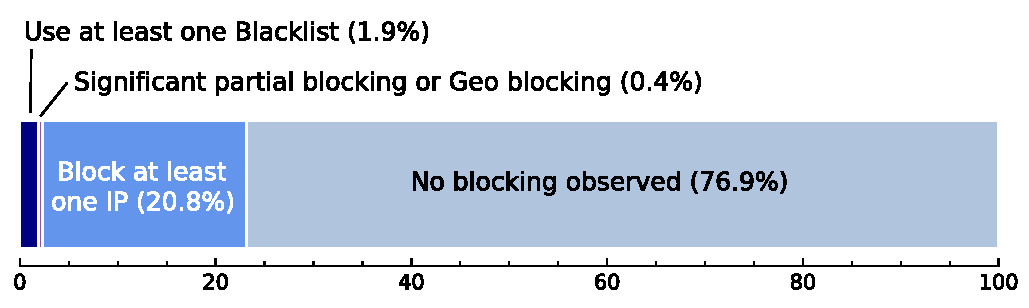
\includegraphics[width=0.95\columnwidth]{data_usage/images/reflector_breakdown_v2.pdf}
\caption{Breakdown of {\reflector} blocking based on three
  experimental runs.}
\label{fig:reflector-breakdown}
\end{figure}

For a particular experimental run, I randomly selected 25 IPs from
each blacklist that satisfies the requirements defined in
Section~\ref{sec:methodology}: exclusive, stable, routable,
geo-diversified, and AS disjoint. Then I evaluated the blocking
behavior for all {\reflroughnum} {\reflectors} against the 225
blacklist IPs sampled from all nine blacklists. To increase the chances
that these sampled IP will be stable, also to handle cases where reflectors
might update the blacklists slowly(a reflector might take a long time to
start blocking the newest IPs in a blacklist, although I discover
later that it is not the case, see Section~\ref{sec:latency-analysis}),
I ensure the sampled IPs have stayed in the blacklist for at least
2 weeks before the experiment. Since for each blacklist,
an experimental run can takes days to perform, as a post-processing step
I remove blacklist IPs from consideration that did not remain on the
blacklist for the duration of the experiment.

To increase the amount of evidence of blacklist blocking behavior, I
conducted three experimental runs, each time using a different set of 25
IPs from each blacklist. I then conclude that a {\reflector} is using a 
blacklist if only if all experiment runs show that it blocked all the 
sampled stable IPs from that blacklist.

I conducted the measurements from December 3--23rd, 2019.  During
this period, I tested 96,067,051 distinct \texttt{\small
  ({\reflector},IP)} pairs\footnote{The first two experiment I tested against
  all {\reflectors}, the last experiment I only tested against the ones that
  have shown blocking behavior in the first two tests}.
Based upon the criteria from
Section~\ref{sec:methodology}, I are able to conclusively determine
the blocking behavior (blocking or not blocking) of 98.3\% of the
tested pairs.  Among these pairs, 894,570 pairs display a
clear signal indicating ``blocking''.

Figure~\ref{fig:reflector-breakdown} presents the blocking behavior of
all 222,782 reflectors I tested partitioned into four categories:
those reflectors that I conclude use at least one of the public
blacklists (1.9\%), reflectors that block a large fraction of IPs on
at least one blacklist in every experiment(0.4\%, see more in
Section~\ref{sec:partial-blocking}), remaining reflectors that block at
least one blacklist IP (20.8\%), and reflectors that do not block any
blacklist IPs (76.9\%). (I identified 4,253 {\reflectors} that use at
  least one blacklist (Section~\ref{sec:blacklist-use}).  I also
  discovered reflectors that block a significant fraction of blacklist
  IPs, due in part to geo-blocking
  (Section~\ref{sec:partial-blocking}).  Finally, I identified a
  large number of reflectors blocking at least one IP, suggesting
  wider use of a much larger set of blacklists
  (Section~\ref{sec:large-scale}).) Note that given the requirements for hosts to
be reflectors, such as running old OS versions, it is not surprising a
large percentage shows no blocking of the blacklist IPs: they already
have attributes anti-correlated with high degrees of security hygiene.
Consequently, I want to emphasize that one should not conclude that
this percentage is representative of all hosts on the Internet.

These high-level results provide the foundation for additional
analyses and experiments, and going forward I further investigate
each of these categories of reflector blocking behavior in turn.
Section~\ref{sec:blacklist-use} explores blacklist use among the
{\reflectors}, Section~\ref{sec:partial-blocking} then examines
significant partial blocking behavior (including geo-blocking), and
Section~\ref{sec:large-scale} explores how reflectors that show any
blocking behavior can be used as evidence of much broader use of
blacklists.  As a final analysis, Section~\ref{sec:consistency}
studies the consistency of reflector blocking behavior at a coarser
granularity.

\begin{table}
\setlength{\tabcolsep}{4pt}
\centering
\caption{The number of {\reflectors} I conclude using each of the nine different
  blacklists, as well as the number of unique /24s and ASes those
  reflectors appear in.}
\begin{tabular}{l r r r}
 \toprule
 \textbf{Blacklist} (abbr.)   & \textbf{Reflectors}  & \textbf{/24s}   & \textbf{ASes}\\
 \midrule
 {\spamhausdrop} (DROP)                  & 4,142         & 1,782  & 50  \\
 {\spamhausedrop} (eDROP)                & 1,272         & 362    & 25  \\
 {\dshieldtop} (DTop)                    & 223           & 69     & 18  \\
 {\etcompromised} (ET)                   & 116           & 58     & 15  \\
 {\bdsatif} (BDS)                        & 85            & 41     & 3   \\
 {\feodo} (Feodo)                        & 64            & 26     & 16  \\
 %\textbf{\ciarmy}                              & 59            & 39 \\
 {\snortfilter} (Snort)                  & 52            & 20     & 11  \\
 {\blocklistde} (DE)                     & 36            & 18     & 8   \\
 {\ettor} (Tor)                          & 24            & 9      & 8   \\
 \midrule
 \textbf{Total Unique}                   & 4,253         & 1,827  & 77  \\
 \bottomrule
\end{tabular}

\label{tab:perfect-blocking-reflectors}
\end{table}

\section{Reflectors Using Blacklists}
\label{sec:blacklist-use}

In this section, I focus on the reflectors that use the blacklists I
study, including the relative popularity of the blacklists, patterns
in the use of multiple blacklists, and the rate at which reflectors
update.  I also use external sources of ground truth to validate my
findings.  Overall, I conclude from the results in this section that
my methodology is indeed effective at identifying blacklist use from
a remote third-party vantage point.

Recall that I use three experimental runs that test whether
reflectors block 25 randomly chosen IPs from the blacklists, and only
conclude that a reflector uses a blacklist if it blocks {\em all}
stable IPs on that blacklist across all runs.  Based on these criteria,
I identified 4,253 reflectors that use one of these public
blacklists.  Table~\ref{tab:perfect-blocking-reflectors} shows the
number of {\reflectors} using each of the nine different blacklists,
as well as the number of unique /24s and ASes those reflectors appear
in.

{\spamhausdrop} is by far the most popular blacklist in the
collection, followed by {\spamhausedrop}.  The remaining blacklists
have a comparatively small number of {\reflectors} using them.  On one
hand, since many aspects of my methodology and experiment make
conservative choices, these results should be considered a lower
bound.  On the other, one should have very high confidence in these results:
I believe these reflectors are actually on networks that block the
IPs on these blacklists.


\begin{figure}[t]
  \centering
  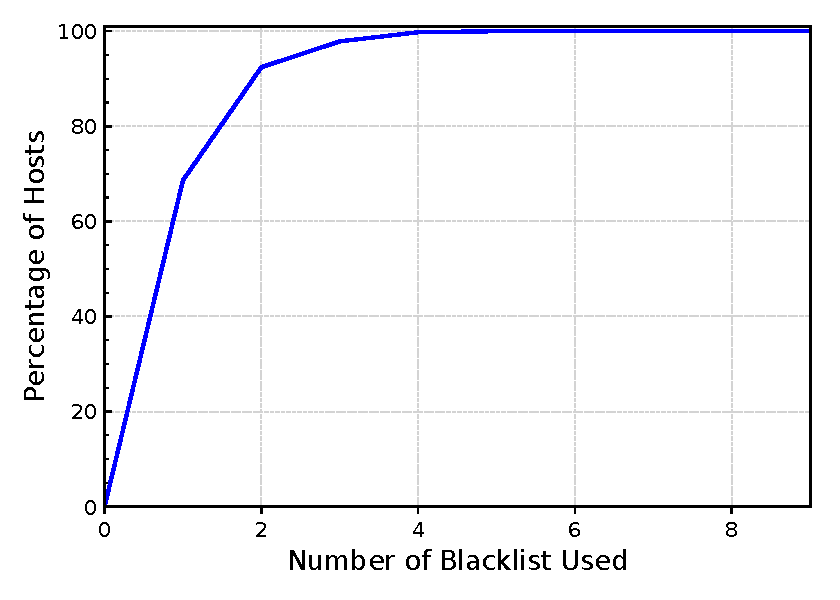
\includegraphics[width=0.8\linewidth]{data_usage/images/perfect_shared_cdf_v2.pdf}
  \caption{CDF of the number of blacklists used by {\reflectors}}
  \label{fig:perfect-shared-cdf}
\end{figure}

\subsection{Multiple Blacklist Use}

For the {\reflectors} using at least one blacklist,
Figure~\ref{fig:perfect-shared-cdf} shows the cumulative distribution
of the number of blacklists they use.  At least for the most popular
public blacklists I study, most use just one.  Over 68.6\% use just
one blacklist, 23.8\% use two or more, and only 7.6\% use three or more.
I find one {\reflector} using six of the nine blacklists -- the most
I see in my study.

For these {\reflectors}, though, there are interesting patterns to the
multiple blacklists used.  Figure~\ref{fig:perfect-heatmap} shows the
use of multiple blacklists with a heatmap.  Each cell shows the fraction of the {\reflectors} using the blacklist in the
   row $R$ that are also using the blacklist in the column $C$: $|R \cap C| / |R|$. Rows and columns
correspond to blacklists, and each cell of the heatmap shows the
fraction of the {\reflectors} using the blacklist in row $R$ that are
also using the blacklist in column $C$.  For example, the first cell
for {\etcompromised} shows that 78\% of the {\reflectors} that use ET
also use the {\spamhausdrop} blacklist.  Diagonal cells are 1.00 since
they show blacklists compared with themselves.

The first cell of the {\spamhausedrop} row indicates that all
{\reflectors} that use {\spamhausedrop} also use {\spamhausdrop}.
Since the eDROP list is an extension of the DROP list, the behavior is
strongly consistent with expectations (and, as such, is also a minor
validation of the methodology).  Moreover, the many significant values
in the first two columns show that {\reflectors} that use any of the
other blacklists very often also use {\spamhausdrop} and eDROP.  These
results underscore the popularity of {\spamhausdrop}, and indicate
that if a {\reflector} blocks traffic using blacklists, it very likely
uses {\spamhausdrop}.

\begin{figure}[t]
  \centering
  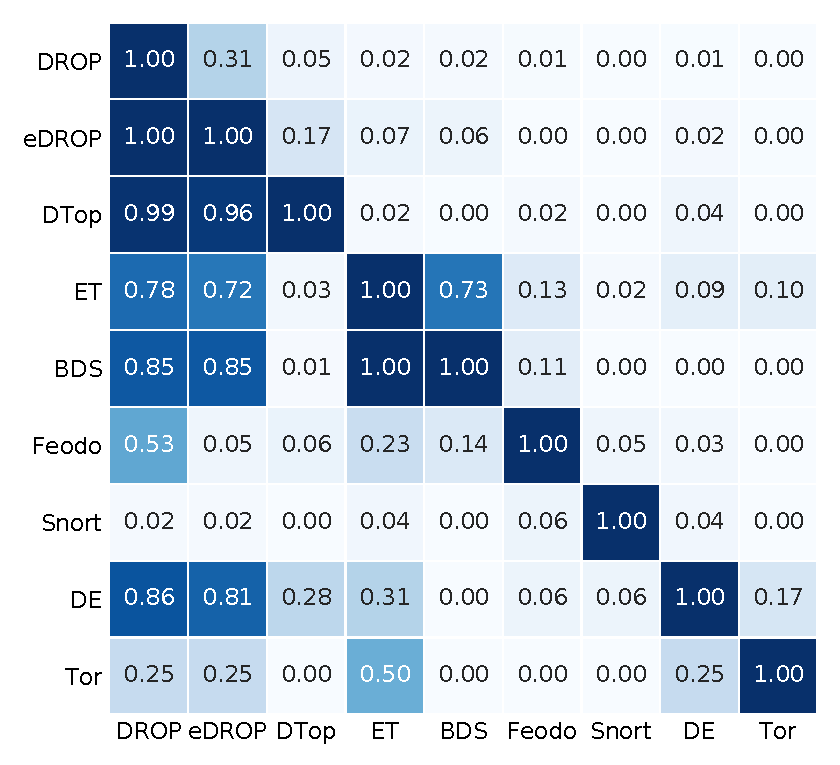
\includegraphics[width=0.85\linewidth]{data_usage/images/perfect_blocking_heatmap.pdf}
  \caption{Pair-wise overlap of {\reflectors} using the different blacklists.}
  \label{fig:perfect-heatmap}
\end{figure}

\subsection{Reflector Update Latency}
\label{sec:latency-analysis}

The objective of IP blacklists is to capture the most up-to-date IPs
associated with malicious activities. As new threats come and go on
the Internet, the content on the lists keeps changing. This dynamic
nature of underlying threats and thus the IPs on the blacklists
underscores the importance of {\reflectors} keeping their blacklists
recent.
%% Thus far, we focused on the stable portion of the blacklist,
%% in order to infer usage.
The goal of our next experiment is to estimate the delay between when
new IPs appear on a blacklist and when reflectors start blocking them.

%% However, to infer update behavior of
%% {\reflectors} we use IPs that are newly added to the blacklist so as
%% to measure how long it takes for {\reflectors} to start blocking the
%% new IPs. We refer this analysis as \textit{latency} analysis.

%% The latency analysis is time sensitive and to get fine granularity
%% we would need to determine the blocking behavior quickly. However,
%% our inference technique is not an instant test. The measurement
%% infrastructure and ethical considerations constrains how quickly
%% we finish the experiment. Typically, the measurement lasts
%% in the order of hours -- allowing us to measure ``latency'' at a
%% day granularity.

%Furthermore, when testing mulitple blacklist IPs against one host, these
%experiments have to be run sequentially, one after another. Otherwise, the
%effects of probing packets on the IP ID field will be mixed together. Also,
%we need to have some gap between each experiment, ensuring different
%experiments will not interfere with each other. All these requirements can
%make one measurement to take hours to finish, making it insufficient to be
%used to reason fine-granularity latency. Therefore, in this experiment we
%focus on day-granularity latency, where we %check how many days do it take
%for each {\reflector} to start blocking newly added IPs %in blacklists.

Because a single pass of the full set of {\reflectors} takes hours, we
examine the blacklist update behavior of {\reflectors} at the
granularity of a day.  For each blacklist we identify newly added IPs
between two consecutive days, and consider only those new IPs that
were not on the blacklist in the prior two weeks.  For this
measurement, the blacklist IPs do not need to be exclusive, but still
need to be routable.  One day after the new IPs appear on a blacklist,
we then test whether the {\reflectors} using that blacklist now block
these IPs, we repeat the experiment daily afterward if necessary.
We also conduct this latency experiment twice to ensure consistent
results(Since {\ettor} is a synthesized list, we did not measure
the update latency regarding this blacklist).

%% After curating this list of blacklist IPs to measure we wait
%% for 24 hours and check if the {\reflectors} we identified in the
%% previous section block these IPs. If no blocking behavior is
%% identified we keep repeating the experiment every day till we see
%% blocking. We repeat this experiment at a later date to ensure
%% consistent results.

%Here we wait for 24 hours because some hosts could update their blacklist
%daily on a fix time (One university we checked update their blacklists every
%day on 6am), then our experiments time might miss the timing.

%% {\dshieldtop},
%% {\etcompromised}, {\bdsatif}, {\bdsatif}, {\feodo}, {\snortfilter},
%% {\blocklistde}, start blocking the newly added IPs on our first measurement
%% indicating that {\reflectors} update their blacklist in a timely manner.

Aside from one outlier, we find that \textit{all} reflectors track
updates to the blacklists. The {\reflectors} that use the six
non-Spamhaus blacklists all update within the one-day period. The
outlier is a group of reflectors using {\spamhausdrop} that stop updating
after late October 2019 (We observed this by testing with the newly added IPs
in {\spamhausdrop} in the past), all the other {\reflectors} that block
{\spamhausdrop} update within one-day period. After investigating, we found that
all these outlier {\reflectors} are located in one organization (a hosting
provider). We suspect this organization stops updating their list after that
October.

For {\spamhausedrop}, it hasn't added new IPs since Dec 17, 2019 as of Feb 14,
2020. We tested all the corresponding {\reflectors} with the newly added IPs
in {\spamhausedrop} back on Dec 17, 2019 and before, and found all the
{\reflectors} are update to date.

%% Thus, in this case we construct lists of ``newly added IPs'' of two
%% list in the past, and check if the {\reflectors} are up to date on
%% these lists.  We find that all {\reflectors} that use {\spamhausedrop}
%% block the set of newly added IPs on December 17th, indicating that
%% these reflectors are up to date. However, in the case of
%% {\spamhausdrop} while most {\reflectors} block the latest newly added
%% IPs, for 2,772 {\reflectors} we find that we need to go before Nov
%% 2019 to find ``newly added IPs'' that are blocked. Mapping the
%% {\reflectors} IPs to an AS and then to an organization using the CAIDA
%% AS to Organization~\cite{caida_as_org} dataset we find that all 2,772
%% {\reflectors} belong to one organization. We suspect this organization
%% included the {\spamhausdrop} on late October 2019 and never updated
%% the list afterwards.

% and strongly
%indicates the use of network level blocking using {\spamhausdrop} by the
%organization.

%, it is a little bit challenging since
%these two lists do not update frequently---only a few times per mont. Worse,
%these new IPs are often unroutable, making them unsuitable for our measurement.
%Therefore, we calculate the newly added IPs in these two lists in the past,
%using the data we collected, and test against the corresponding {\reflectors}.
%We found that all {\reflectors} that use {\spamhausedrop} are blocking the
%latest IPs(added on Dec 17th). While for {\spamhausdrop}, there are 2,772
%{\reflectors} that only blocks IPs that are added earlier than Nov 2019, and
%all the other {\reflectors} are blocking the latest IPs(added on Feb 4th 2020).
%And all these IPs are from the one organization. We suspect this organization
%included the {\spamhausdrop} on late October 2019 and never updated their list.

\subsection{Validation}

We are able to infer the use of blacklists for various hosts from our
measurement. Ideally, we would also want to validate our findings.
After checking the organizations where our {\reflectors} are from, we
reached out to 2 universities that we conclude are using blacklists.
We got the ground truth regarding the exact blacklists they are using, and
successfully validated our findings. More specifically, University $A$
confirmed our findings that they use \bdsatif, \etcompromised,
\spamhausdrop\ and \spamhausedrop. University $B$ confirmed our finding that
they use \spamhausdrop\ and \spamhausedrop.

%For the Tor list blocking, we check the reverse DNS of the {\reflectors},
%and for the ones that we can find the reverse DNS record, we access the website
%from a normal browser and at the same time, from a TOR browser. We observed
%that for all these reflectors, we can access them from a normal browser, but can not
%establish a connection from the Tor browser, proving that they are
%blocking connections from Tor.


\section{Partial Blocking}
\label{sec:partial-blocking}

%% In Section~\ref{sec:perfect-blocking}, we looked into {\reflectors} that
%% consistently block all blacklist IPs sampled for a blacklist. We further
%% confirm this by re-running the measurement three times with three different
%% set of blacklist IPs sampled from the blacklist at different times. However,
%% our measurement also discovers blocking behavior that is not ``perfect''.
%% Every time we sample blacklist IPs and test, many {\reflectors} only block
%% some of the IPs we sampled, while leaving the rest of IPs unblocked. We refer
%% to these cases as \textit{partial blocking}. In this section, we dive deeper
%% into these cases of partial blocking. Specifically, we look at different reasons
%% one may see partial blocking and then look in more detail at {\reflectors}
%% that show consistent, and significant partial blocking.

When performing our experimental runs we noticed that a small
percentage of reflectors consistently blocked a significant subset of
blacklist IPs, but not all, in \textit{every experiment}.
This consistency suggests that, while the
{\reflector} may not use the exact blacklist, there is a large overlap
between the blacklist and the blocking policy of the {\reflector}.  We
refer to such reflectors as exhibiting \textit{significant partial blocking}
behavior.  Figure~\ref{fig:reflector-breakdown} shows these reflectors
are just 0.4\% of all reflectors that we tested, but they still
correspond to 21\% of the number of reflectors that perfectly block at
least one blacklist and therefore motivate further investigation.  As
a result, in this section we characterize this partial blocking
behavior in more detail.

%% Therefore, if a {\reflector} only blocks a small portion of the IPs we
%% sampled from a blacklist, it could not give us much insight about the
%% host's behavior regarding that blacklist.

%% However, we observe that many of these {\reflectors} show partial
%% blocking behavior consistently: Every time we test with a certain
%% blacklist, they always block a significant portion of the IPs we
%% sampled from that list.

%% However, before we dive deeper into these {\reflectors} we briefly touch upon
%% geo-blocking -- a significant contributor to partial blocking and how we try and
%% reduce the effects that geo-blocking may have on our results.
%\textcolor{red}{Show the table about the breakdown between >75\% and >50\%}.

\subsection{Geo-Blocking}
\label{sec:geo-blocking}

%% Geo-blocking is the case where the {\reflector} blocks all the traffic from a
%% certain country. Some sites apply this blocking either for policy reason
%% (e.g. block GDPR countries~\cite{bbcnews}.), or for security reasons (e.g.
%% block countries where recent attacks originated from, like Russia or China).
%% Although during blacklist IP sampling, we go the extra mile to increase the
%% geo diversity of IPs, we might still end up with sampled IPs largely from a
%% few countries. Primarily, this is because the blacklist itself can have a
%% disproportionate amount of IPs from only a few countries. For example,
%% {\dshieldtop} on Jan. 25th had over 50\% of its IPs coming from Netherlands.
%% If a host blocks traffic from Netherlands, then we would miss conclude that
%% host is partially blocking {\dshieldtop}.

%% To eliminate the effects of geo-blocking, we conducted an additional
%% experiment to identify the geo-blocking hosts among our {\reflectors}. For
%% each country the blacklist IPs had covered, we randomly select 20 IPs from
%% that country, and test against all {\reflectors}, using the same IP ID
%% technique, to identify if the hosts that are blocking these IPs. Here we
%% acquire IP address prefixes of each country from 4 location services:
%% MaxMind~\cite{maxmind}, IP2Location~\cite{ip2location}, IPDeny~\cite{ipdeny}
%% and IPIP.net~\cite{ipip}, and we only sample IPs from the intersection of the
%% prefixes provided by each service. Put differently, for each country we test,
%% we only sample from the IPs where all 4 location services are agree they are
%% from that country. We further make sure the sampled IPs are not overlapped
%% with any of the blacklists we have, and they are BGP routable. We tested 20
%% countries in total, from big countries like Russia and China, to small island
%% countries like Singapore and Seychelles.

%% In total, we identify 677 {\reflectors} that at least block one country we
%% tested, and 473 {\reflectors} that block at least two countries. 549
%% {\reflectors} block IPs from China, making it the most popular target of
%% geo-blocking in our collection. Russia is the second most blocked country,
%% where we found 414 hosts blocking Russian IPs, followed by Hong Kong and
%% Vietnam, for which there are 196 and 193 {\reflectors} blocking their IPs
%% respectively. European countries like Belgium, Netherlands and France also
%% have over 60 hosts blocking them.

%% Note that what we discovered here is network layer geo-blocking, and there
%% can be other forms of geo-blocking, like application layer blocking (e.g.
%% HTTP 403 Forbidden). We do not try to comprehensively cover all possible
%% geo-blocking cases since this experiment was only to help us identify the
%% potential side-effects of geo-blocking in our experiment, so we could better
%% distinguish the blacklist related blocking behavior in our experiment.

%% One potential cause of partial blocking is geo-blocking.

Geo-blocking is one type of blocking we identified that contributes to
this partial blocking.  A {\reflector} using geo-blocking will
drop all traffic from a particular country.  Organizations typically
use geo-blocking either for policy reason (e.g., block GDPR
countries~\cite{bbcnews}), or for security reasons (e.g., block
countries that are sources of attacks, such as Russia or China).  If a
reflector uses geo-blocking, we will observe it blocking IPs on a
blacklist if those IPs happen to be located in a blocked country.  Although
we take extra efforts to increase the geo diversity when sampling IPs(Section~\ref{sec:methtarg}),
this kind of overlap can still be exacerbated if a blacklist happens to have
concentrations of IPs from particular countries.  For example,
{\dshieldtop} on January 25, 2020 had over 50\% of its IPs geo-located
in the Netherlands.  If a reflector blocks traffic from the
Netherlands, then we would observe that the reflector is partially
blocking {\dshieldtop}.

%% Recall that Although during blacklist IP sampling, we go the extra
%% mile to increase the geo diversity of IPs, we might still end up with
%% sampled IPs largely from a few countries. Primarily, this is because
%% the blacklist itself can have a disproportionate amount of IPs from
%% only a few countries.

To identify whether a {\reflector} uses geo-blocking, we test whether
the {\reflector} consistently blocks a set of IPs from a particular
country.  For all countries related to blacklist IPs that we test, we
first enumerate the IP address prefixes for those countries using four
IP-based location services: MaxMind~\cite{maxmind},
IP2Location~\cite{ip2location}, IPDeny~\cite{ipdeny}, and
IPIP.net~\cite{ipip}.  For each country, we then randomly select 20 IP
addresses from those prefixes such that: (1) all four location
services agree on the country label for the IPs, (2) the IPs do not
appear on a blacklist, and (3) the IPs are BGP routable.  Then for all
{\reflectors}, we test whether it blocks all of the randomly-chosen
IPs for each country.  If it does, then we conclude that it uses
geo-blocking.

We tested our {\reflectors} against 20 countries in total, ranging
from large countries like Russia and China to small island countries
like Singapore and Seychelles.  Overall, only a small number of
{\reflectors}, 614 (0.28\%), block at least one country, and 432 block
at least two.  China is blocked most often, with 501 of the 614
{\reflectors} blocking random IPs in China.  Russia is second at 376,
followed by Hong Kong (177) and Vietnam (175).  European countries
including Belgium, Netherlands, and France also have over 60
{\reflectors} blocking them.

Note that our methodology identifies geo-blocking at the network
layer.  Other forms of geo-blocking exist, such as application-layer
blocking (e.g., HTTP 403 Forbidden).  We do not explore all possible
geo-blocking mechanisms since our goal was to identify {\reflectors}
using geo-blocking at the network layer.

%% \noteby{GV}{Thinking about it more, if we had more time we could turn
%%   geo-blocking into a result instead of treating it as error.  The
%%   challenge with fitting it into the current framing is that it is not
%%   always significant partial blocking.}

%% , as they could introduce noise
%% when determining network-level blocking based upon blacklists.

\subsection{Significant Partial Blocking}

\begin{table}[t]
\centering
\small
%\begin{adjustbox}{width=\columnwidth}
\begin{tabular}{l r r r | r r r }
 \toprule
 \textbf{}           &\multicolumn{3}{c}{\textbf{Blocked over 75\%}}    &\multicolumn{3}{c}{\textbf{Blocked over 50\%}} \\
 \textbf{Blacklist}  &\textbf{Hosts}   &\textbf{/24s}   &\textbf{ASes}  &\textbf{Hosts}   &\textbf{/24s}   &\textbf{ASes} \\
 \midrule
 DROP      & 28      & 18     & 3   &  23      & 21    & 3\\
 eDROP     & 96      & 60     & 32  &  49      & 27    & 18\\
 DTop        & 157     & 66     & 19  &  319     & 165   & 72\\
 ET     & 13      & 7      & 6   &  31      & 19    & 17\\
 BDS           & 8       & 5      & 5   &  7       & 7     & 7\\
 Feodo             & 65      & 30     & 19  &  23      & 17    & 15\\
 Snort       & 11      & 9      & 7   &  34      & 20    & 17\\
 DE       & 148     & 38     & 1   &  13      & 11    & 4\\
 Tor             & 63      & 35     & 26  &  31      & 19    & 16\\
 %% {\spamhausdrop}      & 28      & 18     & 3   &  23      & 21    & 3\\
 %% {\spamhausedrop}     & 96      & 60     & 32  &  49      & 27    & 18\\
 %% {\dshieldtop}        & 157     & 66     & 19  &  319     & 165   & 72\\
 %% {\etcompromised}     & 13      & 7      & 6   &  31      & 19    & 17\\
 %% {\bdsatif}           & 8       & 5      & 5   &  7       & 7     & 7\\
 %% {\feodo}             & 65      & 30     & 19  &  23      & 17    & 15\\
 %% {\snortfilter}       & 11      & 9      & 7   &  34      & 20    & 17\\
 %% {\blocklistde}       & 148     & 38     & 1   &  13      & 11    & 4\\
 %% {\ettor}             & 63      & 35     & 26  &  31      & 19    & 16\\
 \midrule
 \textbf{Total}              & 492     & 207    & 71  & 459      & 257   & 108\\
 \bottomrule
\end{tabular}
%\end{adjustbox}
\caption{Number of reflectors exhibiting significant partial blocking on each blacklist.}
\label{tab:partial-blocking-reflectors}
\end{table}

%\noteby{GV}{At what point in the workflow are geo-blocking reflectors
%  removed?}

%% Recall that we selected all {\reflectors} exclusively within the US to
%% minimize blocking behavior caused by censorship
%% (Section~\ref{sec:methrefl}).

In addition to geo-blocking, there are reasons why a {\reflector} may
block a blacklist IP that is not due to the reflector using that
blacklist.  A host may have internal policies that deny access from
some network providers, or network administrators may add IPs into
their firewall on an ad-hoc basis based on an organization's internal
strategies or policies.  These alternate blocking behaviors could
overlap with the blacklist IPs we sampled, leading to partial blocking
behavior in our results.

%% We go through all partial blocking we observed, and remove the ones
%% that caused by geo-blocking.

Having identified reflectors using geo-blocking, we remove these
reflectors from further consideration.  We then calculate two groups of
{\reflectors}: for each blacklist, we identify {\reflectors} that
partially block over 75\% of our sampled IPs \textit{every time} we
test them, and another group where they partially block over 50\% of
our sampled IPs.
%We exclude the cases where we fail to conclude the blocking behavior of a
%few {\reflectors} and blacklist IP pairs (after 15 trials)
%\noteby{GV}{Not clear on this?}.

%Every time we test, we sample IPs from the exclusive part of that blacklist,
%where we check against over 100 public IP blacklist (including some obsolete
%ones). Therefore,

For each blacklist, Table~\ref{tab:partial-blocking-reflectors}
summarizes the number of {\reflectors} that fall into each category.
If a {\reflector} is blocking more than 75\% of our sampled IPs every
time, it is plausible that the {\reflector} is using a source that is
very similar to the blacklist we tested.  For instance, there could be
other blacklists where the data collection methodology is similar to
the method used by the public blacklists in our study.  Previous work
has shown that commercial products can aggregate data from public
blacklists, and that they potentially conduct post-processing to
eliminate some content~\cite{li2019reading}.

We suspect that the partial blocking behavior in
Table~\ref{tab:partial-blocking-reflectors} likely results from such
cases.  In particular, the number of {\reflectors} that are partial
blocking {\dshieldtop} is relatively high compared with other
blacklists---it covers over 30\% of all {\reflectors} in the first
group and over 69\% in the second group, suggesting that this list may
be relatively frequently included into other lists.

%% Looking into the organizations related to these partial blocking hosts
%% (Section~\ref{sec:perfect-blocking}), {\feodo} is again covered by the
%% most diverse set of organizations, showing its popularity among
%% different sectors.  \noteby{GV}{Keep in mind that the next section
%%   claims that we cannot map to organizations...}

%% Overall, though, only a small number of {\reflectors} show significant
%% partial blocking, which is consistent with the finding in the previous
%% section.

%% (Less is More)
%% One interesting fact is that there are 253 {\reflectors} from
%% the two partial blocking groups overlap with the {\reflectors} we
%% identified previously that use a blacklist, which is because some
%% {\reflectors} use one blacklist but only partially block another.

\section{Beyond Our Blacklists}
\label{sec:large-scale}

%In this section we analyze how fast does different network update their blocking policy.
%So far the goal of our measurement was to infer if a {\reflector} uses a
%specific blacklist to block traffic. While this informs our view of the usage
%of specific blacklists it does not inform our broader perspective on the
%usage of threat intelligence at large. Essentially, in this section we would
%like to see if any of our {\reflectors} use any blacklist, or implement any
%security features that involves IP-based traffic blocking.

%During our measurement, we looked at over 100 public IP blacklists, but there
%is a wide selection of commercial blacklists that we cannot cover. In order
%to look at the blocking behavior from a wider lens, we would like to test
%blacklist IPs that are shared by as many products as possible. Of course,
%there is no concrete way to identify these IPs, so we try to use some
%heuristic to increase the likelihood that the IPs selected are also covered
%by other blacklists.

%In order to accomplish this, we still sample IPs from the top 9 blacklist we
%identified, but instead of selecting exclusive IPs, we sample from the
%\textit{nonexclusive} portion of each blacklists, so that these IPs are
%shared with at least one more blacklist. We further reduce the candidate pool
%by only keeping the IPs that have stayed in the blacklist for at least 3
%weeks. Being ``shared'' and ``stable'' are the heuristics we use to increase
%the chances that these IPs are also shared with many other blacklists. We
%then drop the IPs that are not routable or are from the {\reflector} AS.
%Finally, we randomly sample 80 IPs from the remaining IPs for our experiment.
%We test these IPs against all our {\reflectors} to identify blocking
%behaviors. To be conservative, we conduct this experiment twice and use two
%different set of randomly selected 80 IPs. Additionally, each time we also
%include a control group, where we randomly select 80 IPs from
%\textcolor{red}{Explain how control group come.}

\begin{figure}[t]
\centering
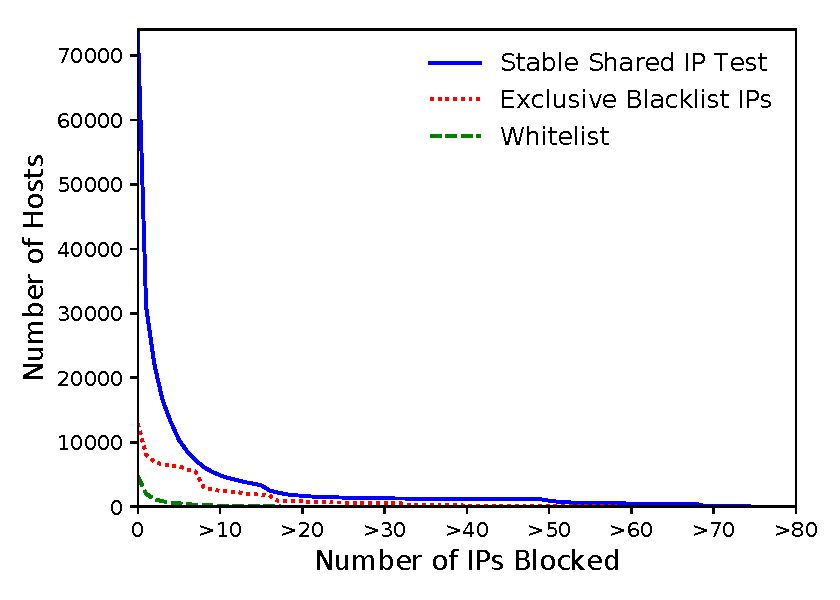
\includegraphics[width=1.0\columnwidth]{images/large_scale_rcdf_v2.pdf}
\caption{Number of {\reflectors} ($y$-axis) that block at least
  some number of blacklist IPs ($x$-axis).  5,412 reflectors,
  for instance, block 10 or more ``Shared'' IPs.}
\label{fig:large_scale_rcdf}
\end{figure}


Previously we chose blacklist IPs that were exclusive to each
blacklist, effectively creating a set of IPs that served as a
signature for that blacklist. But as we can see from Figure~\ref{fig:reflector-breakdown},
there are over 20\% of {\reflectors} that blocked at least one
blacklist IP during one of the three experiments, and we do not
have a clear explanation. One possible case is that the blacklist IPs
we sampled happen to overlap with some commercial blacklists we
do not know, and those lists are more widely used. To check this
possibility, we change our blacklist IP sampling criteria and conduct
a new experiment.

Now our goal is the opposite: we want
to choose among common, or shared, IPs that appear on multiple
blacklists.  As added caution, we also focus on shared IPs that are
the most stable, appearing on the blacklists for at least three weeks.
Our goal is to bias selecting blacklist IPs that are so egregiously
suspicious that not only do they appear on multiple of our public
blacklists for a long period of time, but as a result they also likely
appear on other public and commercial blacklists that we do not have
access to.

% \noteby{GV}{Opportunity for an analogy here.}

For this experiment we randomly selected 80 blacklist IPs that appear
on more than one blacklist and, as with previous experiments, that are
routable and AS disjoint.  We refer to this set as the ``Shared''
blacklist IPs.  For comparison, we also randomly selected a set of 80
blacklist IPs from our previous experiment, the ones that are
exclusive to one blacklist (``Exclusive''), and a random set of 80 IPs
as a whitelist set (``Whitelist''), again with the routable and AS disjoint
criteria. Here the whitelist is constructed by randomly sampling IPs
from top 10,000 most visited IPs among all the network traffic in our own
organization in one day (an education institute of over 30K students
and faculty).


%% This is showed as the green dash line in Figure~\ref{fig:large_scale_rcdf}.

For each of these sets of 80 blacklist IPs,
Figure~\ref{fig:large_scale_rcdf} shows how many {\reflectors} block
the same number of IPs as a distribution over the number of blacklist
IPs blocked.  (We evaluated multiple random sets of shared blacklist
IPs to see whether the random selections introduced noticeable
variance.  Since the results were very consistent across the different
random sets, for clarity we just show results for one of them.)  For
example, for ``Exclusive'' blacklist IPs only 2,649 {\reflectors}
block 10 or more IPs.  In contrast, for ``Shared'' blacklist IPs that
appear on more than one blacklist, far more {\reflectors} block them.
Over 73K {\reflectors} block at least one IP from the shared set, and
5,412 {\reflectors} block 10 or more IPs.  In contrast, for the
whitelist set, there are only 202 {\reflectors} that block 10 or more
whitelist IPs(we checked these whitelist IPs and found the most blocked
ones are from Cloudflare, which is a popular CDN network but
known to associate with malicious activities).
These results suggest that the number of Internet
hosts that potentially use security-related traffic blocking is much
larger than just the ones that use the public blacklists we study.

%% \noteby{GV}{Since shared 1 and 2 essentially overlap, we can just show
%%   one on the graph.  I added the footnote to convey that we did this
%%   more than once for added reassurance.}\noteby{VL}{I still feel it
%%   is a little bit weird if we do not show both result in the graph, because in
%%   the following we say we use top 12 IPs in \textbf{two} experiments}.

%% Uses a larger font size
\begin{table}[t]
\centering
\small
\begin{tabular}{r  r  r  r}
 \toprule
                         & \multicolumn{3}{c}{\textbf{Granularity}} \\
 \textbf{Blacklist IP}   & \textbf{IP}  & \textbf{/24}   & \textbf{AS}\\
 \midrule
 178.73.215.171             & 25,749                 & 175        & 210     \\
 185.176.27.98              & 15,560                 & 5,598      & 1,690   \\
 185.175.93.103             & 13,550                 & 1,155      & 1,224   \\
 92.63.194.115              & 11,889                 & 2,028      & 1,442   \\
 176.10.99.200              & 9,049                  & 466        & 238     \\
 185.156.73.54              & 8,863                  & 1,623      & 5,441   \\
 80.67.223.41               & 6,689                  & 624       & 624      \\
 176.100.109.3              & 4,871                  & 553       & 610      \\
 171.25.193.25              & 4,468                  & 212       & 148      \\
 216.239.90.19              & 4,421                  & 56        & 39       \\
 185.220.102.8              & 4,297                  & 273       & 273      \\
 62.210.37.82               & 4,058                  & 528       & 300      \\
 \bottomrule
\end{tabular}
\caption{Blocking behavior of reflectors with the top 12 most-blocked
  blacklist IPs.  The second column shows the number of {\reflectors}
  that block the particular IP, the third column shows the
  \textit{maximum} number of {\reflectors} that block IPs from the
  same /24, and the last column shows the maximum number of
  {\reflectors} that block IPs sampled from the same AS.}
\label{tab:super-malicious-ips}
\end{table}


% (probably should have the %s in separate columns for more convenient column space control)
\begin{table*}[t]
	\centering
	\small
	\begin{tabular}{l|rr|r|r} \toprule
		\multicolumn{1}{c}{\textbf{}} & \multicolumn{2}{c}{\textbf{Consistent}}                                                      & \multicolumn{1}{c}{\textbf{Almost Consistent}} & \multicolumn{1}{c}{\textbf{Inconsistent}}      \\
		\textbf{Blacklist}            & \multicolumn{1}{c}{\textbf{No Blocking (\%)}} & \multicolumn{1}{c|}{\textbf{Consistent (\%)}} & \multicolumn{1}{c|}{\textbf{Off By One (\%)}}   & \multicolumn{1}{c}{\textbf{Inconsistent (\%)}} \\
\midrule
{\bdsatif} & 35,540 \hspace*{2pt} (88.19\%) & 398 \hspace*{2pt} (0.99\%) & 2,332 \hspace*{2pt} (5.79\%) & 2,030 \hspace*{2pt} (5.03\%) \\
{\blocklistde} & 40,228 \hspace*{2pt} (99.82\%) & 24 \hspace*{2pt} (0.06\%) & 13 \hspace*{2pt} (0.03\%) & 35 \hspace*{2pt} (0.09\%) \\
{\dshieldtop} & 39,603 \hspace*{2pt} (98.27\%) & 393 \hspace*{2pt} (0.98\%) & 138 \hspace*{2pt} (0.34\%) & 166 \hspace*{2pt} (0.41\%) \\
{\etcompromised} & 39,535 \hspace*{2pt} (98.10\%) & 298 \hspace*{2pt} (0.74\%) & 102 \hspace*{2pt} (0.25\%) & 365 \hspace*{2pt} (0.91\%) \\
{\feodo} & 39,943 \hspace*{2pt} (99.11\%) & 195 \hspace*{2pt} (0.48\%) & 42 \hspace*{2pt} (0.10\%) & 120 \hspace*{2pt} (0.31\%) \\
{\snortfilter} & 39,830 \hspace*{2pt} (98.83\%) & 250 \hspace*{2pt} (0.62\%) & 88 \hspace*{2pt} (0.22\%) & 132 \hspace*{2pt} (0.33\%) \\
{\spamhausdrop} & 39,320 \hspace*{2pt} (97.57\%) & 750 \hspace*{2pt} (1.86\%) & 30 \hspace*{2pt} (0.07\%) & 200 \hspace*{2pt} (0.50\%) \\
{\spamhausedrop} & 39,792 \hspace*{2pt} (98.73\%) & 349 \hspace*{2pt} (0.87\%) & 36 \hspace*{2pt} (0.09\%) & 123 \hspace*{2pt} (0.31\%) \\
{\ettor} & 40,000 \hspace*{2pt} (99.25\%) & 165 \hspace*{2pt} (0.41\%) & 43 \hspace*{2pt} (0.11\%) & 92 \hspace*{2pt} (0.23\%) \\
\midrule
\textbf{Overall} & 353,791 \hspace*{2pt} (97.54\%) & 2,822 \hspace*{2pt} (0.78\%) & 2,824 \hspace*{2pt} (0.78\%) & 3,263 \hspace*{2pt} (0.90\%) \\
\midrule
\textbf{Control Group} & 40,255 \hspace*{2pt} (99.89\%)	& 3 \hspace*{2pt} (0.01\%) & 37 \hspace*{2pt} (0.09\%) & 5 \hspace*{2pt} (0.01\%) \\
\bottomrule
	\end{tabular}
	\caption{The blocking consistency of the reflectors in /24 prefixes with more than one reflector.  Multiple reflectors in most /24 prefixes do not block, and as such are consistent.  But when multiple reflectors in /24 prefixes do block, there is substantial inconsistency.  }
	\label{tab:consistency-breakdown}
\end{table*}

Of course, it is possible that this more extensive blocking behavior
is not a result of security-related blocking, but rather because of
other blocking policies such as geo-blocking.  One notable difference,
though, is that security-based traffic blocking usually targets
individual IPs, whereas other policy-driven blocking can target a
specific network or subnet.  As another experiment, we check whether
the blocking we observed indeed targets individual IPs, or instead
larger network blocks.  We select the top 12 IPs where they have
the most amount of {\reflectors} blocking them in the previous test.
For each of these blacklist IPs, we randomly sample
another three IPs from the same /24, and randomly sample another four
IPs from the same AS.  For all of these IPs, we then measure how many
{\reflectors} block each of them.

%% (Original version)
%%
%% \begin{table}[t]
%% \centering
%% \footnotesize
%% \begin{tabular}{r | r | r | r}
%%  \toprule
%%  \textbf{Blacklist IP}   & \textbf{Blocking IP}  & \textbf{Blocking /24}   & \textbf{Blocking AS}\\
%%  \midrule
%%  178.73.215.171             & 25,749                 & 175        & 210     \\
%%  185.176.27.98              & 15,560                 & 5,598      & 1,690   \\
%%  185.175.93.103             & 13,550                 & 1,155      & 1,224   \\
%%  92.63.194.115              & 11,889                 & 2,028      & 1,442   \\
%%  176.10.99.200              & 9,049                  & 466        & 238     \\
%%  185.156.73.54              & 8,863                  & 1,623      & 5,441   \\
%%  80.67.223.41               & 6,689                  & 624       & 624      \\
%%  176.100.109.3              & 4,871                  & 553       & 610      \\
%%  171.25.193.25              & 4,468                  & 212       & 148      \\
%%  216.239.90.19              & 4,421                  & 56        & 39       \\
%%  185.220.102.8              & 4,297                  & 273       & 273      \\
%%  62.210.37.82               & 4,058                  & 528       & 300      \\
%%  \bottomrule
%% \end{tabular}
%% \caption{Blocking behavior of reflectors with the top 12 most-blocked
%%   blacklist IPs.  The second column shows the number of {\reflectors}
%%   that block the particular IP, the third column shows the
%%   \textit{maximum} number of {\reflectors} that block IPs from the
%%   same /24, and the last column shows the maximum number of
%%   {\reflectors} that block IPs sampled from the same AS.}
%% \label{tab:super-malicious-ips}
%% \end{table}


Table~\ref{tab:super-malicious-ips} shows the number of {\reflectors}
that block the top 12 blacklist IPs, the random IPs from the same
/24 as the blacklist IPs, and the random IPs from the same AS (For the
/24 test and AS test, we listed the maximum number of {\reflectors} that
block IPs in two tests). These
results confirm that {\reflectors} exhibit blocking behavior targeting
specific IPs rather than larger network blocks.  Indeed, searching the
Web based on these blacklist IPs returns reports linking these IPs to
a range of malicious activities, including massive port scanning,
brute-force login attempts, and sending spam. That said, although we do
not know the exact feeds these hosts are using, our results suggest
that security-related network blocking is prevalent even among hosts
such as these reflectors.

\section{Blocking Consistency}
\label{sec:consistency}
% TODO: Location of the Table! :(
% GEOFF: Link to the breakdown by AS Type
% https://docs.google.com/spreadsheets/d/1QAWr1qb01reJVAmhvl-ukOJjDl5E_1kr_uIQrAOwWyo/edit#gid=691238820
%
%% \begin{table*}[t]
%% 	\centering
%% 	\small
%% 	\begin{tabular}{l|rr|r|r} \toprule
%% 		\multicolumn{1}{c}{\textbf{}} & \multicolumn{2}{c}{\textbf{Consistent}}                                                      & \multicolumn{1}{c}{\textbf{Almost Consistent}} & \multicolumn{1}{c}{\textbf{Inconsistent}}      \\
%% 		\textbf{Blacklist}            & \multicolumn{1}{c}{\textbf{No Blocking (\%)}} & \multicolumn{1}{c}{\textbf{Consistent (\%)}} & \multicolumn{1}{c}{\textbf{Off By One (\%)}}   & \multicolumn{1}{c}{\textbf{Inconsistent (\%)}} \\ \hline
%% 		\textbf{\bdsatif}              & 35540 (88.19\%)                               & 398 (0.99\%)                                 & 2332 (5.79\%)                                  & 2030 (5.03\%)                                  \\
%% 		\textbf{\blocklistde}          & 40228 (99.82\%)                               & 24 (0.06\%)                                  & 13 (0.03\%)                                    & 35 (0.09\%)                                    \\
%% 		\textbf{\dshieldtop}           & 39603 (98.27\%)                               & 393 (0.98\%)                                 & 138 (0.34\%)                                   & 166 (0.41\%)                                   \\
%% 		\textbf{\etcompromised}        & 39535 (98.10\%)                               & 298 (0.74\%)                                 & 102 (0.25\%)                                   & 365 (0.91\%)                                   \\
%% 		\textbf{\feodo}                & 39943 (99.11\%)                               & 195 (0.48\%)                                 & 42 (0.10\%)                                    & 120 (0.31\%)                                   \\
%% 		\textbf{\snortfilter}          & 39830 (98.83\%)                               & 250 (0.62\%)                                 & 88 (0.22\%)                                    & 132 (0.33\%)                                   \\
%% 		\textbf{\spamhausdrop}         & 39320 (97.57\%)                               & 750 (1.86\%)                                 & 30 (0.07\%)                                    & 200 (0.50\%)                                   \\
%% 		\textbf{\spamhausedrop}        & 39792 (98.73\%)                               & 349 (0.87\%)                                 & 36 (0.09\%)                                    & 123 (0.31\%)                                   \\
%% 		\textbf{\ettor}                & 40000 (99.25\%)                               & 165 (0.41\%)                                 & 43 (0.11\%)                                    & 92 (0.23\%)                                    \\
%% 		\midrule
%% 		\textbf{Overall} 			   & 353791 (97.54\%)   & 2822	(0.78\%) & 2824 (0.78\%) & 3263 (0.90\%) \\
%% 		\midrule
%% 		\textbf{Control Group}  	   & 40255  (99.89\%)	& 3	(0.01\%)	& 37 (0.09\%)	 & 5 (0.01\%)	   \\
%% 		\bottomrule
%% 	\end{tabular}
%% 	\caption{Consistency Breakdown}
%% 	\label{tab:consistency-breakdown}
%% \end{table*}

As a final analysis, we explore the consistency of reflector blocking
behavior at a coarser granularity.  A common use case of blacklists is
at the granularity of an organization, often via some kind of network
appliance.  In such a scenario, we would expect the blocking behavior
of {\reflectors} to be consistent across an organization: if one
{\reflector} blocks a blacklist IP, then other {\reflectors} in the
same organization should also block it.

Ideally we would like to map reflectors to organizations to answer
this question.  However, mapping an IP to an organization is a
challenging problem, particularly with the increasing use of WHOIS
anonymization.  Instead, we use the common, more tractable technique
of aggregating reflectors by their /24 prefix.  As a result, in this
section we answer a methodological question: If we aggregate
reflectors by their /24 prefix, do the aggregated reflectors exhibit
consistent blocking behavior?  Is the /24 prefix aggregation a useful
proxy for expected consistent blocking by organizations?

%% However, mapping an IP to an organization is a
%% challenging problem, particularly with the increasing use of WHOIS
%% anonymization.  Further, multiple ``organizations'' could potentially
%% map to a single AS, as with transit and access ASes. Thus, we use the
%% common method of assuming hosts on the same /24 prefix are part of the
%% same network and, as such, the same organization.

%% Specifically, for each /24 with more than one {\reflector}, we check
%% if the {\reflectors} block the exact same set of sampled blacklist IPs.

%\subsection{Consistency Methodology}

Our data set has 134,370 {\reflectors} that are part of /24s with more
than one {\reflector}.  For each blacklist, we categorize the blocking
behavior of multiple {\reflectors} in the same /24 into one of three
categories: \textit{consistent}, \textit{almost consistent}, and
\textit{inconsistent}.  We define a /24 to be ``consistent'' for a
blacklist if \textit{all} the individual {\reflectors} in that /24
block the \textit{exact same} blacklist IPs.
%
A /24 is ``almost consistent'' if the blocking behavior of the
{\reflectors} in a /24 differs only by one IP. For example, a /24 is
``almost consistent'' if it has four {\reflectors}, three of which
block the same 21 IPs from a blacklist, and the fourth {\reflector}
blocks 20 out the same 21 IPs.
%% since if we had tried more than 15 times we could have potentially
%% found them to be consistent.
%
Finally, we consider all other /24s ``inconsistent''.

%% any /24 that does not fall into the aforementioned two categories,
%% we consider them as ``inconsistent''.

%there is the case of missed blacklist IPs -- blacklist IPs for which we could
%not get a good signal for blocking behavior. In the specific instance, where
%the sum of ``perfect'' and ``missed'' blacklist IPs is exactly the same for
%all individual {\reflectors} in a /24 we carve out that /24 as unknown since
%had we persisted beyond 15 tries we could have found it as consistent.

%\subsection{Consistency Results}

Using these definitions, Table~\ref{tab:consistency-breakdown} shows
the consistency results for all the /24s that have more than one
{\reflector}.  The results are dominated by /24s that do not show any
blocking behavior.  We consider such /24s consistent since all the
hosts under these /24s block the same number (zero) of blacklist IPs,
but these cases also do not provide much insight.

Excluding the ``no blocking'' cases, then in the presence of any
blocking, consistency of blocking behavior at a /24 granularity is far
from guaranteed.  As discussed in Section~\ref{subsec:fpfn_analysis},
our measurement technique has very low false positive and false
negative rates.  Measurement error can potentially explain some
``almost consistent'' cases and perhaps some ``inconsistent'' cases,
too.  However, the consistency results for the control group,
comprised of 20 randomly sampled US IPs
(Section~\ref{sec:perfect-blocking}), shows that the potential effect
of measurement error on consistency is small.  In other words, the
inconsistent cases do indeed demonstrate different blocking behavior
among hosts within the same /24.

One situation that could lead to inconsistent blocking behavior within
a /24 is when the network belongs to a cloud or hosting provider, and
the IPs within the same /24 are used by distinct entities.  For
instance, when manually examining the inconsistent /24s for {\bdsatif}
(which has the highest inconsistency), we found more than 60\% of
these /24s belong to cloud or hosting providers.  Another situation
leading to inconsistent block behavior is when a /24 belongs to an ISP
which sub-allocates IP addresses to different customers.

In summary, our results indicate that we cannot assume consistent
blocking behavior for {\reflectors} in the same /24 network.



%\section{Discussion}


\subsection{Limitation}
%Our measurement took the first step to understand how threat intelligence
%blacklists are used on the Internet.
Our experiment took the first to unveil how threat intelligence blacklists are
used on the Internet, by measuring over 220K hosts on the Internet. One
limitation of our measurement, however, is the hosts we selected. We select
these hosts primarily based on the present of IP ID side channel, and low
network traffic. This might affect our candidate selection, provide us a biased
set of sample set. We provide a lower bound for the threat intelligence usage
online.

Another limitation is our limited access to the commercial threat intelligence
products. All the experiment in this paper is conducted with public threat
intelligence feeds. As we see from Section~\ref{sec:partial-blocking} and
Section~\ref{sec:large-scale}, the potential number of hosts that are using
some threat intelligence products is much higher. In this paper, we took the
best effort to peer into the commercial space, relying on the fact that some
commercial products share content with public feeds. Future work should explore
more the commercial threat intelligence.


\subsection{Future Work}
Our work try to understand the usage of threat intelligence products. We utilize
the IP ID side channel and measured one specific type of usage: network layer
traffic blocking. But as we mentioned earlier, there are many different ways
people can use the threat intelligence, future work should focusing more on
unveiling other type of usage, for example, application layer access deny.

Another thing regarding the IP ID side channel is that although the global
shared IP ID counter is regarded as old implemention, and more recent system
have switched to more modern implementions. But as pointed out by~\cite{klein2019ip},
even the most recent IP ID implementation still consist of exploitable side
channels. Future work could explore the possibility to using these side channels,
to create more vantage points for this type of measurement.

\section{Conclusion}
Our paper describes, implements and tests a technique for inferring
the deployment of network layer blacklisting and, further, for
attributing the use of particular blacklists in particular networks.
There are a range of limitations in our pilot study, most
significantly including potential selection bias arising from using
quiescent U.S. hosts running older versions of Windows as well as our
exclusive use of public blacklist data (i.e., we do not have access to
high-priced commercial threat intelligence feeds which could be
distinct).  However, even given these limitations our measurements of
220K hosts reveal a number of interesting artifacts.  First, we
witness the widespread use of \emph{some} kind of network layer
blocking (affecting over a third of hosts in our data set) even if it
is not consistent with membership in any of the lists we track.
Second, we find that there is evidence of intra-network diversity in
traffic blocking policy.  While a number of network prefixes have
consistent blocking behavior across multiple hosts, quite a few do
not, suggesting different network security policies are being employed
on different subnets.  Finally, for blacklist use that can be
precisely attributed the most widely used blacklists (Spamhaus DROP
and eDROP and DShield Top) are also those that have extremely low
false positives.~\footnote{The DROP and eDROP lists are a small subset
  of Spamhaus' feed that specifically deals with address for which the
  entire network prefix is believed to be abusive (e.g., prefix
  hijacking).} This suggests that for many networks proactive traffic
  blocking is gated on having lists of sufficient accuracy to remove
  the risks of accidentally blocking legitimate traffic.
